% \documentclass[9pt, aspectratio=169]{beamer}
\documentclass[9pt]{beamer}
\usepackage[utf8]{inputenc}
\usepackage{graphicx}
\usepackage{amsmath,amssymb,amsfonts}
\usepackage{tikz}
\usepackage{caption}
\usepackage{epstopdf}
%\usepackage[table]{xcolor}
% \usepackage{case}
%\usepackage{matlab}
\usefonttheme[onlymath]{serif}



\usetheme{Madrid}
\usecolortheme{default}


% \usetheme{AnnArbor}
% \usecolortheme{default}

\usepackage{caption}
\captionsetup{font=footnotesize}


%\AddToHook{shipout/foreground}{
%    \ifnum\thepage>1
%        \begin{tikzpicture}[overlay, remember picture]
%            \node[text=black, rotate=0, scale=1, opacity=0.1] at (current page.center) 
%                {
\includegraphics[width=0.5\paperwidth]{logo.png}};
%        \end{tikzpicture}
%    \fi
%}




%------------------------------------------------------------
%This block of code defines the information to appear in the
%Title page
\title[Underwater Vehicles]{Underwater Vehicles}
\subtitle{Modeling, }

% \subtitle{2D model}

\author[D.C. Vu] % (optional) 
{Duc Cuong Vu}

\institute [MEG, MoCAR, HUST]
{
  \textit{Motion Control and Applied Robotics Laboratory,}\\
  School of Electrical and Electronic Engineering,\\
  Hanoi University of Science and Technology\\
}

\date[Ver. 1.0, \today] {Version: 1.0\\ Last updated: \today}

\logo{
\includegraphics[height=0.8cm]{logo}}

%------------------------------------------------------------
%The next block of commands puts the table of contents at the 
%beginning of each section and highlights the current section:

\AtBeginSection[]
{
  \begin{frame}
    \frametitle{Table of Contents}
    \tableofcontents[currentsection]
  \end{frame}
}
%------------------------------------------------------------


\begin{document}
\fontsize{9}{13}\selectfont
%The next statement creates the title page.
\frame{\titlepage}


%---------------------------------------------------------
%This block of code is for the table of contents after
%the title page
\begin{frame}
\frametitle{Table of Contents}
\tableofcontents
\end{frame}
%---------------------------------------------------------





\section{Introduction}
% =========================================
% =========================================




\begin{frame}{Introduction}
	\framesubtitle{Handbooks and references}
	UUV - Unmanned Underwater vehicle
	\begin{figure}
		\centering
		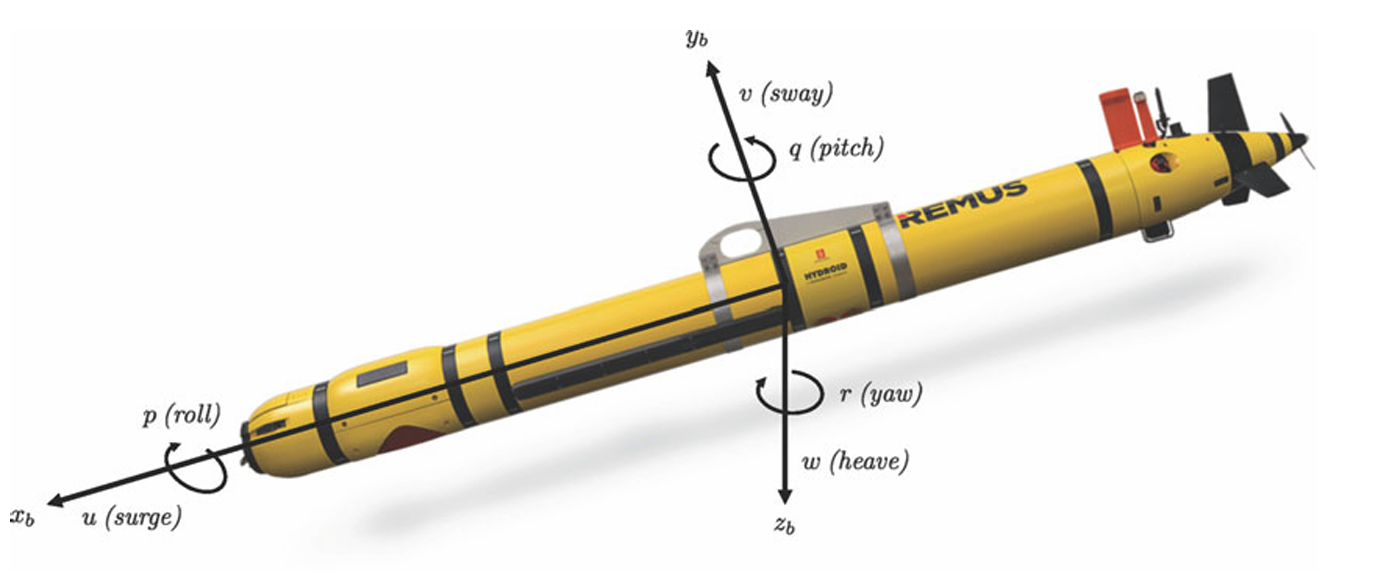
\includegraphics[width=0.75\linewidth]{img/6DOF motion AUV}
		\caption{6-DOF motion variables for a UUV/AUV}
		\label{fig: UUV}
	\end{figure}
	
	Handbooks \& References:
	\begin{itemize}
		\item Thor I. Fossen, \textit{Handbook of Marine Craft Hydrodynamics and Motion Control}, Wiley, 2011.
		\item Thor I. Fossen, \textit{Guidance and Control of Ocean Vehicles}, Wiley, 1994.
	\end{itemize}
	
\end{frame}

% =========================================
% =========================================




\begin{frame}{Introduction}
	\framesubtitle{Handbooks and references}
	\begin{tikzpicture}[remember picture,overlay]
		% \node[fill=blue!30, text=white, font=\large, rounded corners] 
		\node at (current page.north east) [xshift=-11cm, yshift=-3.5cm] 
		{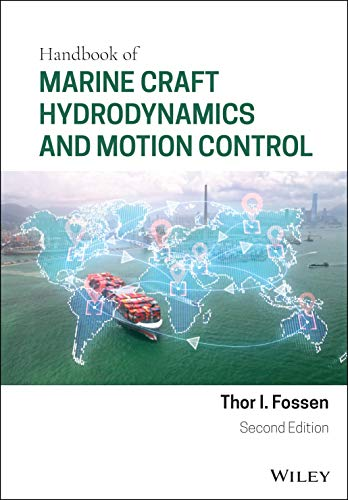
\includegraphics[width=0.23\linewidth]{img/handbook.png}};
	\end{tikzpicture}
	
	\begin{tikzpicture}[remember picture,overlay]
		% \node[fill=blue!30, text=white, font=\large, rounded corners] 
		\node at (current page.north east) [xshift=-8cm, yshift=-3.5cm] 
		{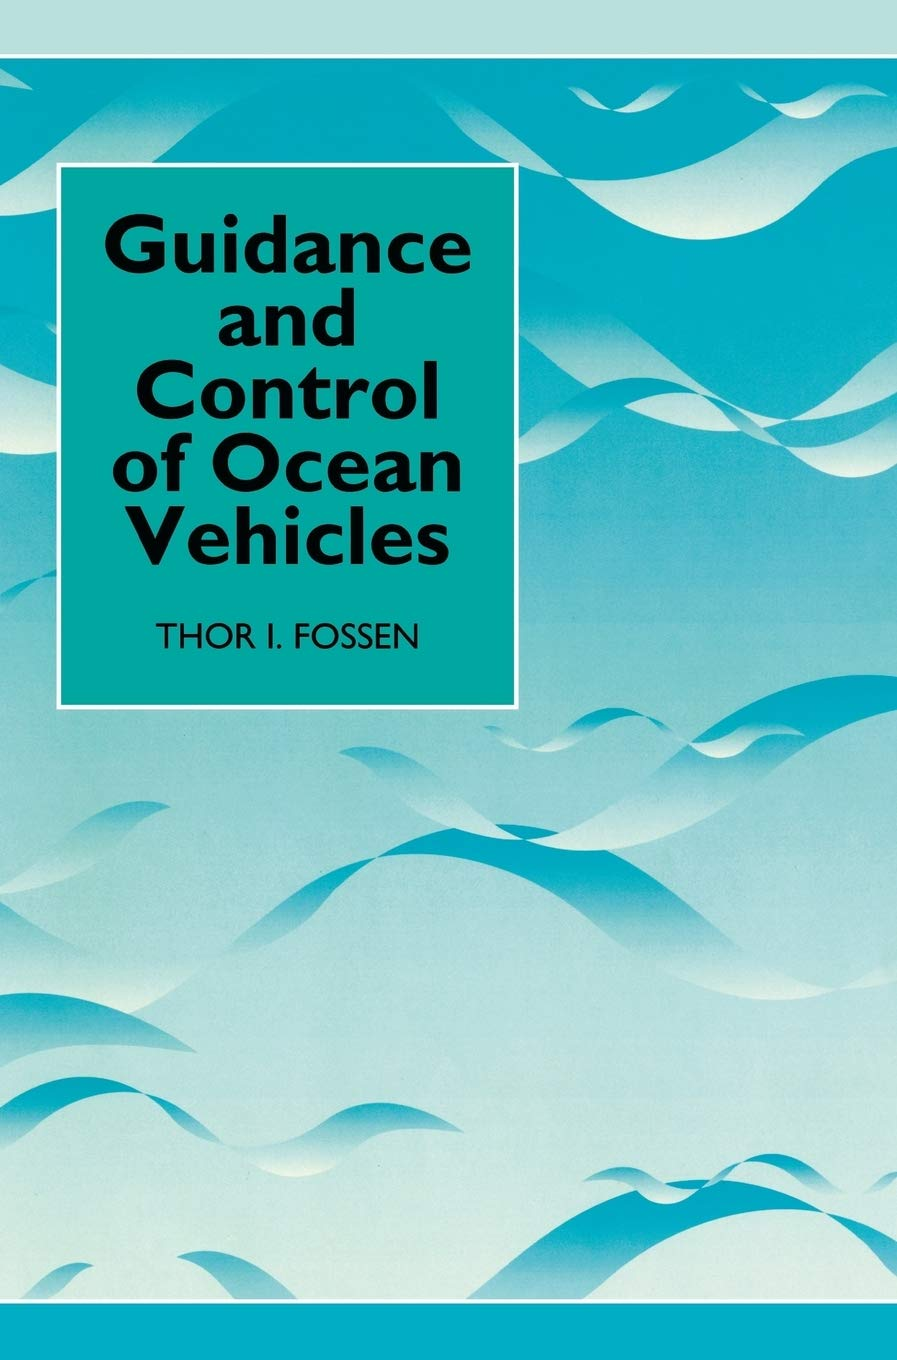
\includegraphics[width=0.23\linewidth]{img/handbook1.png}};
	\end{tikzpicture}
	
	\begin{tikzpicture}[remember picture,overlay]
		% \node[fill=blue!30, text=white, font=\large, rounded corners] 
		\node at (current page.north east) [xshift=-5cm, yshift=-3.5cm] 
		{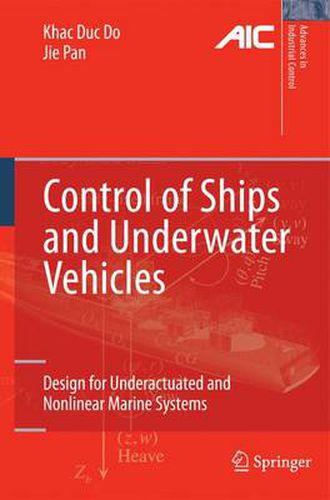
\includegraphics[width=0.23\linewidth]{img/handbook2.png}};
	\end{tikzpicture}
	
	\begin{tikzpicture}[remember picture,overlay]
		% \node[fill=blue!30, text=white, font=\large, rounded corners] 
		\node at (current page.north east) [xshift=-2cm, yshift=-3.5cm] 
		{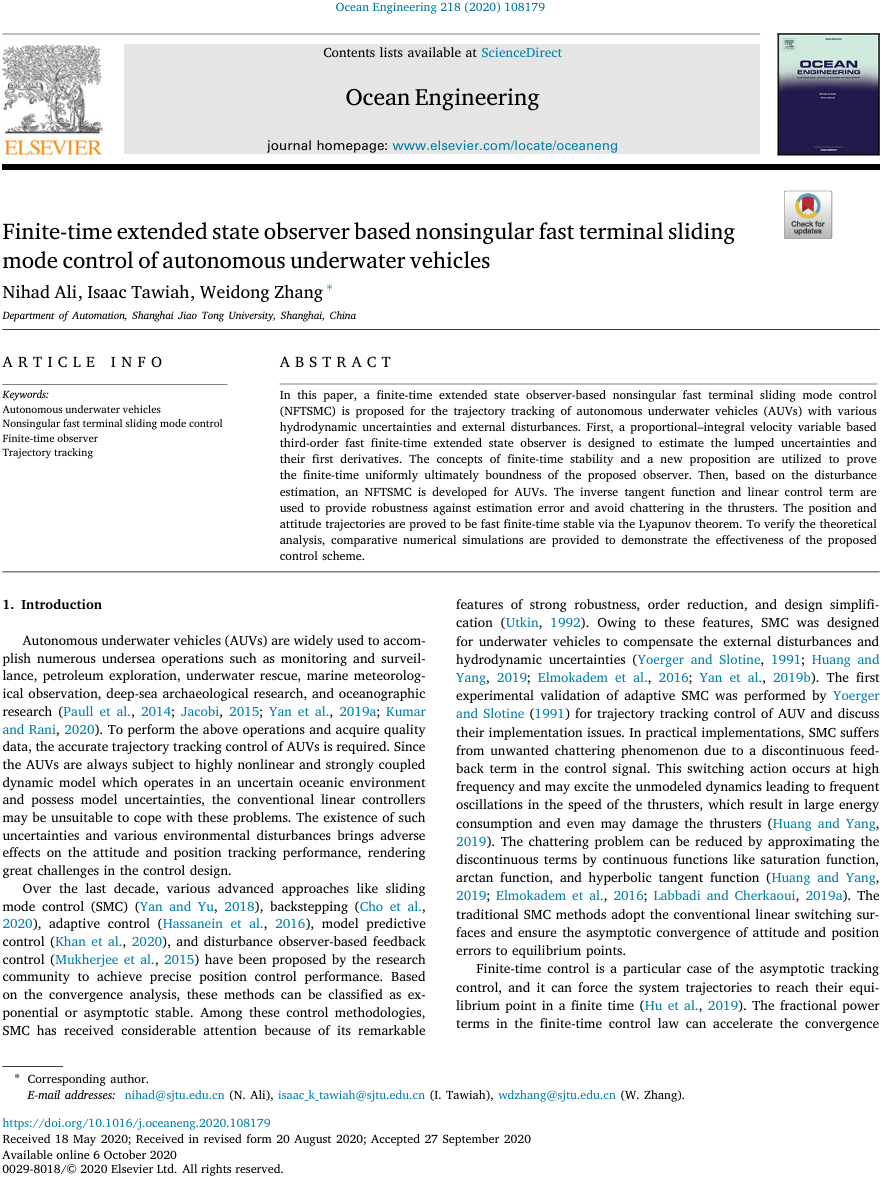
\includegraphics[width=0.23\linewidth]{img/handbook4.png}};
	\end{tikzpicture}
	
	
	
	\vspace{2cm}
	
	Handbooks \& References:
	\begin{itemize}
		\item Review articles, Research articles, Handbook, ...
		\item IEEE Explore, Springer, Elserview, Wiley, Taylor \& Francis, ...
	\end{itemize}
	
\end{frame}

% =========================================
% =========================================




\begin{frame}{Introduction}
	\framesubtitle{Automatic Weather Routing}
	\centering
	\scalebox{0.8}{

\tikzset{every picture/.style={line width=0.75pt}} %set default line width to 0.75pt        

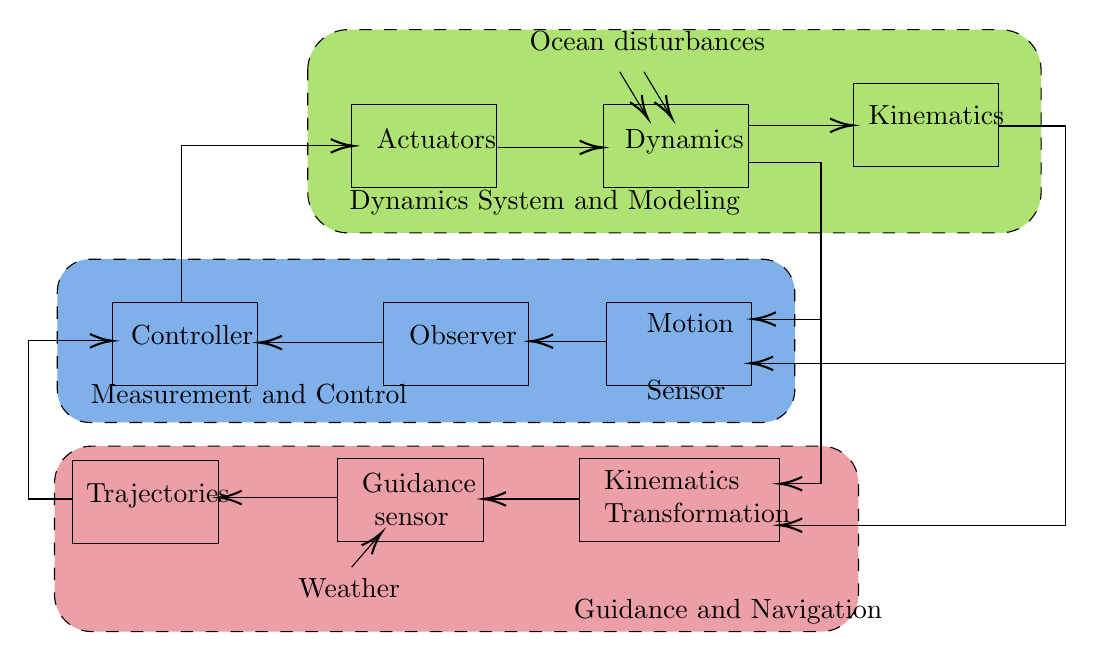
\begin{tikzpicture}[x=0.75pt,y=0.75pt,yscale=-1,xscale=1]
%uncomment if require: \path (0,400); %set diagram left start at 0, and has height of 400

%Rounded Rect [id:dp024716399980995396] 
\draw  [fill={rgb, 255:red, 126; green, 211; blue, 33 }  ,fill opacity=0.63 ][dash pattern={on 4.5pt off 4.5pt}] (224.86,72.14) .. controls (224.86,61.32) and (233.63,52.55) .. (244.44,52.55) -- (558.6,52.55) .. controls (569.42,52.55) and (578.19,61.32) .. (578.19,72.14) -- (578.19,130.9) .. controls (578.19,141.72) and (569.42,150.49) .. (558.6,150.49) -- (244.44,150.49) .. controls (233.63,150.49) and (224.86,141.72) .. (224.86,130.9) -- cycle ;
%Rounded Rect [id:dp820569210963702] 
\draw  [fill={rgb, 255:red, 74; green, 144; blue, 226 }  ,fill opacity=0.71 ][dash pattern={on 4.5pt off 4.5pt}] (104.19,178.89) .. controls (104.19,170.2) and (111.23,163.16) .. (119.92,163.16) -- (443.79,163.16) .. controls (452.48,163.16) and (459.52,170.2) .. (459.52,178.89) -- (459.52,226.09) .. controls (459.52,234.78) and (452.48,241.82) .. (443.79,241.82) -- (119.92,241.82) .. controls (111.23,241.82) and (104.19,234.78) .. (104.19,226.09) -- cycle ;
%Rounded Rect [id:dp6482229762233973] 
\draw  [color={rgb, 255:red, 0; green, 0; blue, 0 }  ,draw opacity=1 ][fill={rgb, 255:red, 208; green, 2; blue, 27 }  ,fill opacity=0.38 ][dash pattern={on 4.5pt off 4.5pt}] (102.86,271.08) .. controls (102.86,261.22) and (110.86,253.22) .. (120.72,253.22) -- (472.32,253.22) .. controls (482.19,253.22) and (490.19,261.22) .. (490.19,271.08) -- (490.19,324.68) .. controls (490.19,334.55) and (482.19,342.55) .. (472.32,342.55) -- (120.72,342.55) .. controls (110.86,342.55) and (102.86,334.55) .. (102.86,324.68) -- cycle ;
%Shape: Rectangle [id:dp008171136473899221] 
\draw   (367.33,88.67) -- (437.33,88.67) -- (437.33,128.67) -- (367.33,128.67) -- cycle ;
%Shape: Rectangle [id:dp578249717098626] 
\draw   (487.67,78.33) -- (557.67,78.33) -- (557.67,118.33) -- (487.67,118.33) -- cycle ;
%Shape: Rectangle [id:dp05994207844147015] 
\draw   (246,88.67) -- (316,88.67) -- (316,128.67) -- (246,128.67) -- cycle ;
%Shape: Rectangle [id:dp3752897955760164] 
\draw   (368.67,183.83) -- (438.67,183.83) -- (438.67,223.83) -- (368.67,223.83) -- cycle ;
%Shape: Rectangle [id:dp9144008780653681] 
\draw   (130.67,183.83) -- (200.67,183.83) -- (200.67,223.83) -- (130.67,223.83) -- cycle ;
%Shape: Rectangle [id:dp6067520460647975] 
\draw   (261.33,183.83) -- (331.33,183.83) -- (331.33,223.83) -- (261.33,223.83) -- cycle ;
%Shape: Rectangle [id:dp21504321988161568] 
\draw   (356,259.33) -- (452,259.33) -- (452,299.33) -- (356,299.33) -- cycle ;
%Shape: Rectangle [id:dp2963684683337764] 
\draw   (239.33,259.33) -- (309.33,259.33) -- (309.33,299.33) -- (239.33,299.33) -- cycle ;
%Shape: Rectangle [id:dp12173800355567699] 
\draw   (111.67,260) -- (181.67,260) -- (181.67,300) -- (111.67,300) -- cycle ;
%Straight Lines [id:da588131875954907] 
\draw    (164.19,183.88) -- (164.19,108.55) -- (244.86,108.55) ;
\draw [shift={(246.86,108.55)}, rotate = 180] [color={rgb, 255:red, 0; green, 0; blue, 0 }  ][line width=0.75]    (10.93,-3.29) .. controls (6.95,-1.4) and (3.31,-0.3) .. (0,0) .. controls (3.31,0.3) and (6.95,1.4) .. (10.93,3.29)   ;
%Straight Lines [id:da637808700504805] 
\draw    (316.47,109.33) -- (364.8,109.33) ;
\draw [shift={(366.8,109.33)}, rotate = 180] [color={rgb, 255:red, 0; green, 0; blue, 0 }  ][line width=0.75]    (10.93,-3.29) .. controls (6.95,-1.4) and (3.31,-0.3) .. (0,0) .. controls (3.31,0.3) and (6.95,1.4) .. (10.93,3.29)   ;
%Straight Lines [id:da38171557543802015] 
\draw    (437.13,98.67) -- (485.47,98.67) ;
\draw [shift={(487.47,98.67)}, rotate = 180] [color={rgb, 255:red, 0; green, 0; blue, 0 }  ][line width=0.75]    (10.93,-3.29) .. controls (6.95,-1.4) and (3.31,-0.3) .. (0,0) .. controls (3.31,0.3) and (6.95,1.4) .. (10.93,3.29)   ;
%Straight Lines [id:da7149208141383911] 
\draw    (437.47,116.67) -- (472.13,116.67) -- (472.13,192) -- (441.47,192) ;
\draw [shift={(439.47,192)}, rotate = 360] [color={rgb, 255:red, 0; green, 0; blue, 0 }  ][line width=0.75]    (10.93,-3.29) .. controls (6.95,-1.4) and (3.31,-0.3) .. (0,0) .. controls (3.31,0.3) and (6.95,1.4) .. (10.93,3.29)   ;
%Straight Lines [id:da9344395667032277] 
\draw    (558,99) -- (590.13,99) -- (590.13,213.33) -- (440.13,213.33) ;
\draw [shift={(438.13,213.33)}, rotate = 360] [color={rgb, 255:red, 0; green, 0; blue, 0 }  ][line width=0.75]    (10.93,-3.29) .. controls (6.95,-1.4) and (3.31,-0.3) .. (0,0) .. controls (3.31,0.3) and (6.95,1.4) .. (10.93,3.29)   ;
%Straight Lines [id:da7282910208505873] 
\draw    (590.13,213.33) -- (590.13,291.33) -- (454.13,291.33) ;
\draw [shift={(452.13,291.33)}, rotate = 360] [color={rgb, 255:red, 0; green, 0; blue, 0 }  ][line width=0.75]    (10.93,-3.29) .. controls (6.95,-1.4) and (3.31,-0.3) .. (0,0) .. controls (3.31,0.3) and (6.95,1.4) .. (10.93,3.29)   ;
%Straight Lines [id:da9182086877003304] 
\draw    (472.13,192) -- (472.13,271.33) -- (454.13,271.33) ;
\draw [shift={(452.13,271.33)}, rotate = 360] [color={rgb, 255:red, 0; green, 0; blue, 0 }  ][line width=0.75]    (10.93,-3.29) .. controls (6.95,-1.4) and (3.31,-0.3) .. (0,0) .. controls (3.31,0.3) and (6.95,1.4) .. (10.93,3.29)   ;
%Straight Lines [id:da9524515432659333] 
\draw    (355.33,278.67) -- (311.47,278.67) ;
\draw [shift={(309.47,278.67)}, rotate = 360] [color={rgb, 255:red, 0; green, 0; blue, 0 }  ][line width=0.75]    (10.93,-3.29) .. controls (6.95,-1.4) and (3.31,-0.3) .. (0,0) .. controls (3.31,0.3) and (6.95,1.4) .. (10.93,3.29)   ;
%Straight Lines [id:da02741576724077044] 
\draw    (238.8,278) -- (184.13,278) ;
\draw [shift={(182.13,278)}, rotate = 360] [color={rgb, 255:red, 0; green, 0; blue, 0 }  ][line width=0.75]    (10.93,-3.29) .. controls (6.95,-1.4) and (3.31,-0.3) .. (0,0) .. controls (3.31,0.3) and (6.95,1.4) .. (10.93,3.29)   ;
%Straight Lines [id:da49199432560322975] 
\draw    (111.8,278.67) -- (90.19,278.67) -- (90.19,202.49) -- (128.86,202.49) ;
\draw [shift={(130.86,202.49)}, rotate = 180] [color={rgb, 255:red, 0; green, 0; blue, 0 }  ][line width=0.75]    (10.93,-3.29) .. controls (6.95,-1.4) and (3.31,-0.3) .. (0,0) .. controls (3.31,0.3) and (6.95,1.4) .. (10.93,3.29)   ;
%Straight Lines [id:da16345135268080146] 
\draw    (368.8,202.67) -- (334.13,202.67) ;
\draw [shift={(332.13,202.67)}, rotate = 360] [color={rgb, 255:red, 0; green, 0; blue, 0 }  ][line width=0.75]    (10.93,-3.29) .. controls (6.95,-1.4) and (3.31,-0.3) .. (0,0) .. controls (3.31,0.3) and (6.95,1.4) .. (10.93,3.29)   ;
%Straight Lines [id:da3511077229754682] 
\draw    (261.52,203.33) -- (203.52,203.33) ;
\draw [shift={(201.52,203.33)}, rotate = 360] [color={rgb, 255:red, 0; green, 0; blue, 0 }  ][line width=0.75]    (10.93,-3.29) .. controls (6.95,-1.4) and (3.31,-0.3) .. (0,0) .. controls (3.31,0.3) and (6.95,1.4) .. (10.93,3.29)   ;

% Text Node
\draw (372,99.2) node [anchor=north west][inner sep=0.75pt]   [align=left] {{\normalfont\selectfont { Dynamics}}};
% Text Node
\draw (489.33,87.87) node [anchor=north west][inner sep=0.75pt]   [align=left] {{\normalfont\selectfont { Kinematics}}};
% Text Node
\draw (387,188.2) node [anchor=north west][inner sep=0.75pt]   [align=left] {\begin{minipage}[lt]{26.74pt}\setlength\topsep{0pt}
{\normalfont\selectfont { Motion}}
\begin{center}
{\normalfont\selectfont { Sensor}}
\end{center}

\end{minipage}};
% Text Node
\draw (268,193.53) node [anchor=north west][inner sep=0.75pt]   [align=left] {{\normalfont\selectfont { Observer}}};
% Text Node
\draw (138.33,193.87) node [anchor=north west][inner sep=0.75pt]   [align=left] {{\normalfont\selectfont {Controller}}};
% Text Node
\draw (252.33,99.2) node [anchor=north west][inner sep=0.75pt]   [align=left] {{\normalfont\selectfont { Actuators}}};
% Text Node
\draw (326,51.87) node [anchor=north west][inner sep=0.75pt]   [align=left] {{\normalfont\selectfont { Ocean disturbances}}};
% Text Node
\draw (112.33,270.2) node [anchor=north west][inner sep=0.75pt]   [align=left] {{\normalfont\selectfont { Trajectories}}};
% Text Node
\draw (214.67,315.53) node [anchor=north west][inner sep=0.75pt]   [align=left] {{\normalfont\selectfont { Weather}}};
% Text Node
\draw (249.67,264.87) node [anchor=north west][inner sep=0.75pt]   [align=left] {\begin{minipage}[lt]{36.02pt}\setlength\topsep{0pt}
{\normalfont\selectfont { Guidance }}
\begin{center}
{\normalfont\selectfont { sensor}}
\end{center}

\end{minipage}};
% Text Node
\draw (366.33,263.87) node [anchor=north west][inner sep=0.75pt]   [align=left] {\begin{minipage}[lt]{53.18pt}\setlength\topsep{0pt}
{\normalfont\selectfont { Kinematics \\ Transformation}}

\end{minipage}};
% Text Node
\draw (347.33,325.53) node [anchor=north west][inner sep=0.75pt]   [align=left] {{\normalfont\selectfont { Guidance and Navigation}}};
% Text Node
\draw (114.67,222.2) node [anchor=north west][inner sep=0.75pt]   [align=left] {{\normalfont\selectfont { Measurement and Control}}};
% Text Node
\draw (239.33,128.87) node [anchor=north west][inner sep=0.75pt]   [align=left] {{\normalfont\selectfont { Dynamics System and Modeling}}};
% Connection
\draw    (386.86,72.87) -- (399.28,93.49) ;
\draw [shift={(400.31,95.2)}, rotate = 238.95] [color={rgb, 255:red, 0; green, 0; blue, 0 }  ][line width=0.75]    (10.93,-3.29) .. controls (6.95,-1.4) and (3.31,-0.3) .. (0,0) .. controls (3.31,0.3) and (6.95,1.4) .. (10.93,3.29)   ;
% Connection
\draw    (375.19,72.87) -- (387.61,93.49) ;
\draw [shift={(388.64,95.2)}, rotate = 238.95] [color={rgb, 255:red, 0; green, 0; blue, 0 }  ][line width=0.75]    (10.93,-3.29) .. controls (6.95,-1.4) and (3.31,-0.3) .. (0,0) .. controls (3.31,0.3) and (6.95,1.4) .. (10.93,3.29)   ;
% Connection
\draw    (246,311.53) -- (259.13,296.38) ;
\draw [shift={(260.44,294.87)}, rotate = 130.91] [color={rgb, 255:red, 0; green, 0; blue, 0 }  ][line width=0.75]    (10.93,-3.29) .. controls (6.95,-1.4) and (3.31,-0.3) .. (0,0) .. controls (3.31,0.3) and (6.95,1.4) .. (10.93,3.29)   ;

\end{tikzpicture}
}
\end{frame}


% =========================================
% =========================================

\begin{frame}{Introduction}
	\framesubtitle{Model classifications}
	Degree of Freedom classifications under purpose
	\begin{itemize}
		\item 1 DOF $\to$ model can be used to design the forward speed controller and heading autopilots and damping system
		\item 3 DOFs $\to$ describe the horizontal plane, longitudinal, and lateral models.
		\item 4 DOFs $\to$ describe the motion in the horizontal plane with heading autopilots and system damping
		\item 6 DOFs $\to$ describe the fully coupled equation of motion used for simulation and prediction.
	\end{itemize}
	
	Naval Architecture
	\begin{itemize}
		\item Maneuvering theory: moving at positive constant speed in calm water
		\item  Seeking theory: motion of ships at zero or constraint speed in waves, which can be analyzed. The hydrodynamic coefficient and wave forces are computed as a function
	\end{itemize}
\end{frame}

% =========================================
% =========================================

\begin{frame}{Introduction}
	\framesubtitle{Tools and Toolboxs}
	\begin{tikzpicture}[remember picture,overlay]
		% \node[fill=blue!30, text=white, font=\large, rounded corners] 
		\node at (current page.north east) [xshift=-4.5cm, yshift=-3cm] 
		{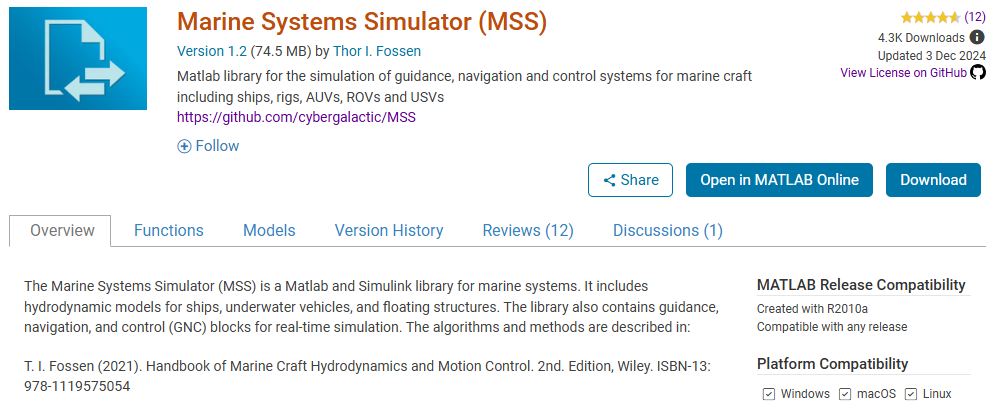
\includegraphics[width=0.7\linewidth]{img/mss toolbox.png}};
	\end{tikzpicture}
	
	\begin{tikzpicture}[remember picture,overlay]
		% \node[fill=blue!30, text=white, font=\large, rounded corners] 
		\node at (current page.north east) [xshift=-4.5cm, yshift=-6.5cm] 
		{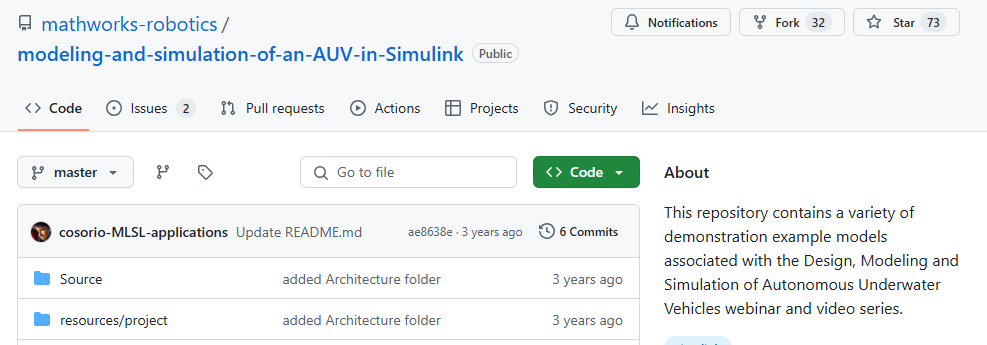
\includegraphics[width=0.7\linewidth]{img/simscape.png}};
	\end{tikzpicture}
	
	
	
	Marine Systems Simulator (MSS) Toolbox \footnote{T. I. Fossen and T. Perez (2004). Marine Systems Simulator (MSS). URL: https://github.com/cybergalactic/MSS} 
	
	\vspace{3cm}
	
	MATLAB Simscape Multibody \footnote{https://github.com/mathworks-robotics/modeling-and-simulation-of-an-AUV-in-Simulink} 
\end{frame}

% =========================================
% =========================================


\begin{frame}{Introduction}
	
	\begin{tikzpicture}[remember picture,overlay]
		% \node[fill=blue!30, text=white, font=\large, rounded corners] 
		\node at (current page.north east) [xshift=-3.8cm, yshift=-3cm] 
		{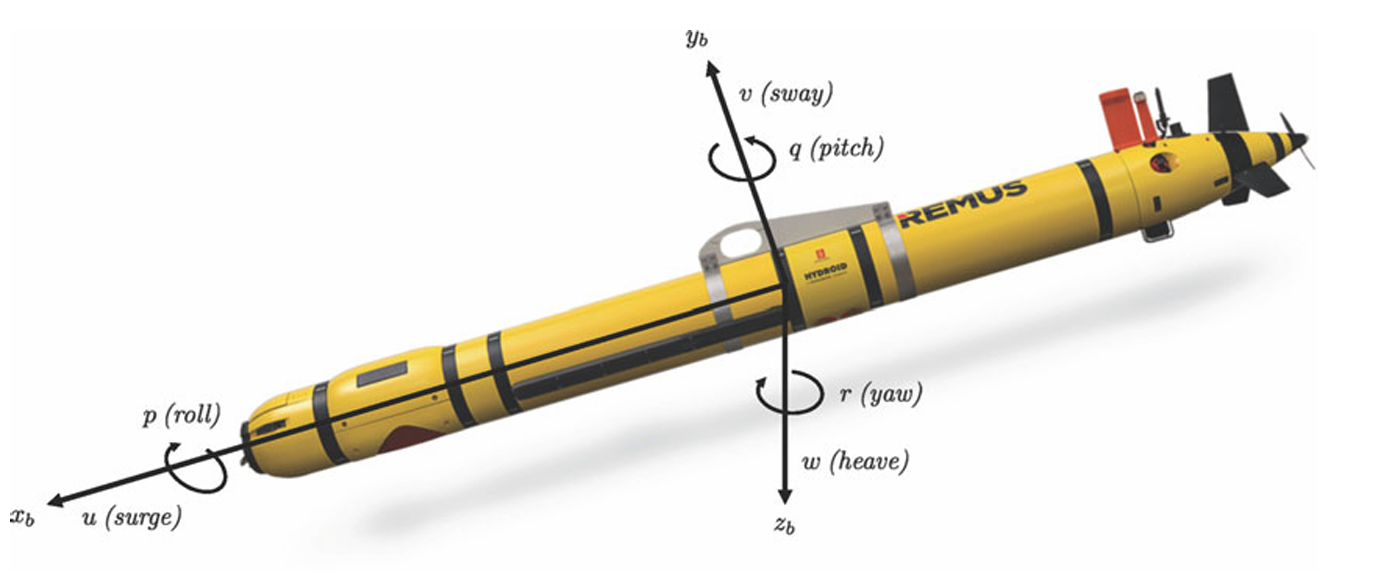
\includegraphics[width=0.7\linewidth]{img/6DOF motion AUV.png}};
	\end{tikzpicture}
	
	\vspace{2cm}
	
	Overview of this seminar
	\begin{itemize}
		\item Fundamental knowledge 
		\item 6-DOF model of a Rigid Body
		\item Ocean dynamics
		\item Environmental disturbances
		\item An example of the ODIN
		\item Guidance - Navigation - Control
		\item Numerical simulations
		\item Quasi-Physical Simulation for UV motion control
		\item An excample for GNC-integrated Quasi-Physical simulation
	\end{itemize}
\end{frame}




% =========================================
% =========================================

\section{Fundamental knowledge}
% =========================================
% =========================================

\begin{frame}{Fundamental knowledge for modeling}
	\framesubtitle{Coordinates}
	
	
	\begin{tikzpicture}[remember picture,overlay]
		\node at (current page.north east) [xshift=-3.5cm, yshift=-4.7cm] 
		{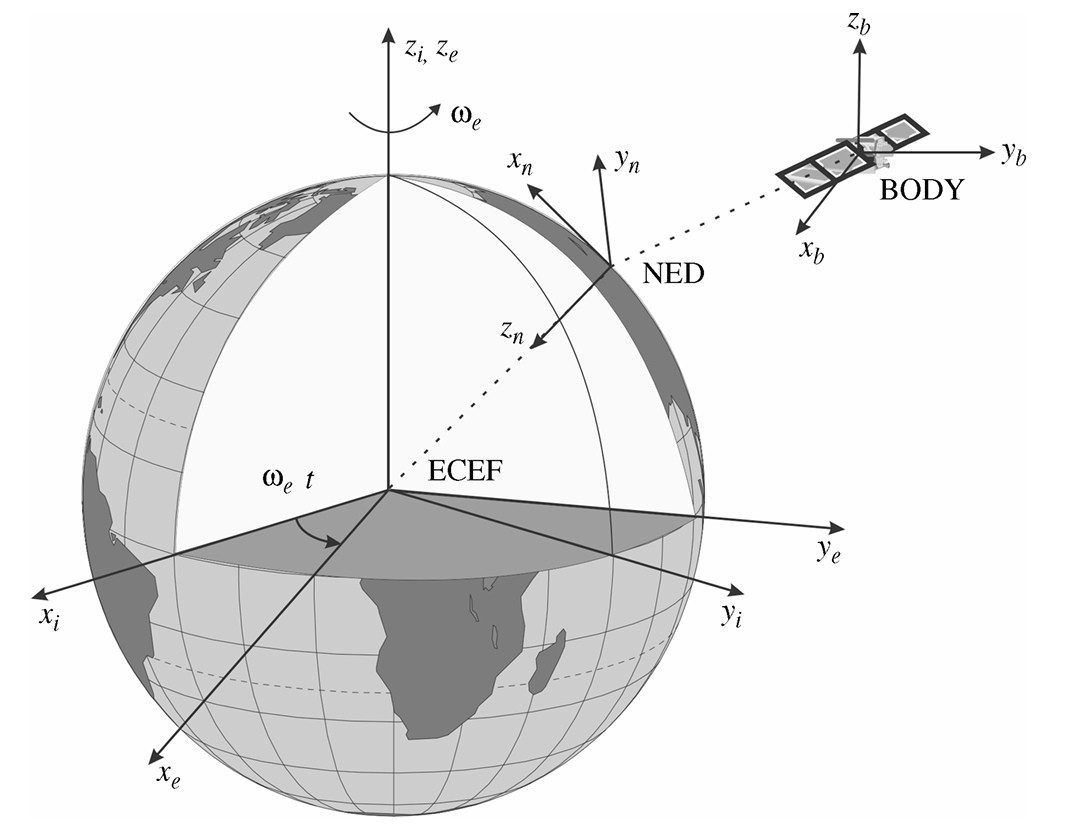
\includegraphics[width=0.6\linewidth]{img/frame.png}};
	\end{tikzpicture}
	
	Earth-Centered reference frames
	\begin{itemize}
		\item ECI - $\{i\}$ - (Earth-centered inertial)
		\item ECEF - $\{e\}$ - (Earth-centered Earth-fixed)
	\end{itemize}
	
	Geographic reference frames
	\begin{itemize}
		\item NED - $\{n\}$ - (North-East-Down)
		\item BODY - $\{b\}$ - (Craft-fixed)
	\end{itemize}
	\vspace{4cm}
	
\end{frame}

% =========================================
% =========================================


\begin{frame}{Fundamental knowledge for modeling}
	\framesubtitle{Coordinates}
	
	
	\begin{tikzpicture}[remember picture,overlay]
		% \node[fill=blue!30, text=white, font=\large, rounded corners] 
		\node at (current page.north east) [xshift=-4cm, yshift=-4.7cm] 
		{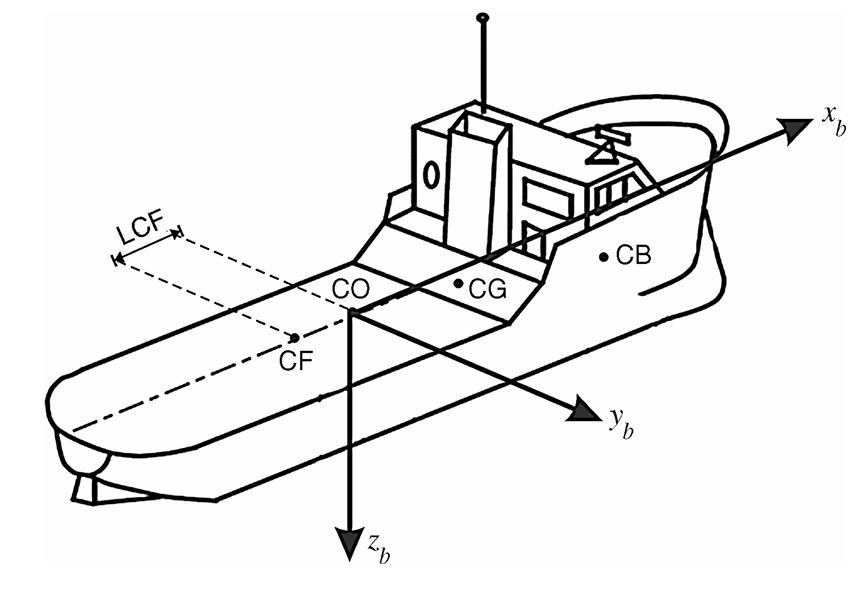
\includegraphics[width=0.65\linewidth]{img/BODY.png}};
	\end{tikzpicture}
	
	The origin of the BODY frame is CO. Then, 
	\begin{itemize}
		\item CG - Center of Gravity
		\item CB - Center of Buoyancy
		\item CF - Center of flotation
	\end{itemize}
	
	\vspace{3cm}
	
	The center of flotation is the centroid of water plane area $A_{wp}$ in calm water.
\end{frame}

% =========================================
% =========================================


\begin{frame}{Fundamental knowledge for modeling}
	\framesubtitle{Notations}
	
	\begin{tikzpicture}[remember picture,overlay]
		% \node[fill=blue!30, text=white, font=\large, rounded corners] 
		\node at (current page.north east) [xshift=-3.8cm, yshift=-3cm] 
		{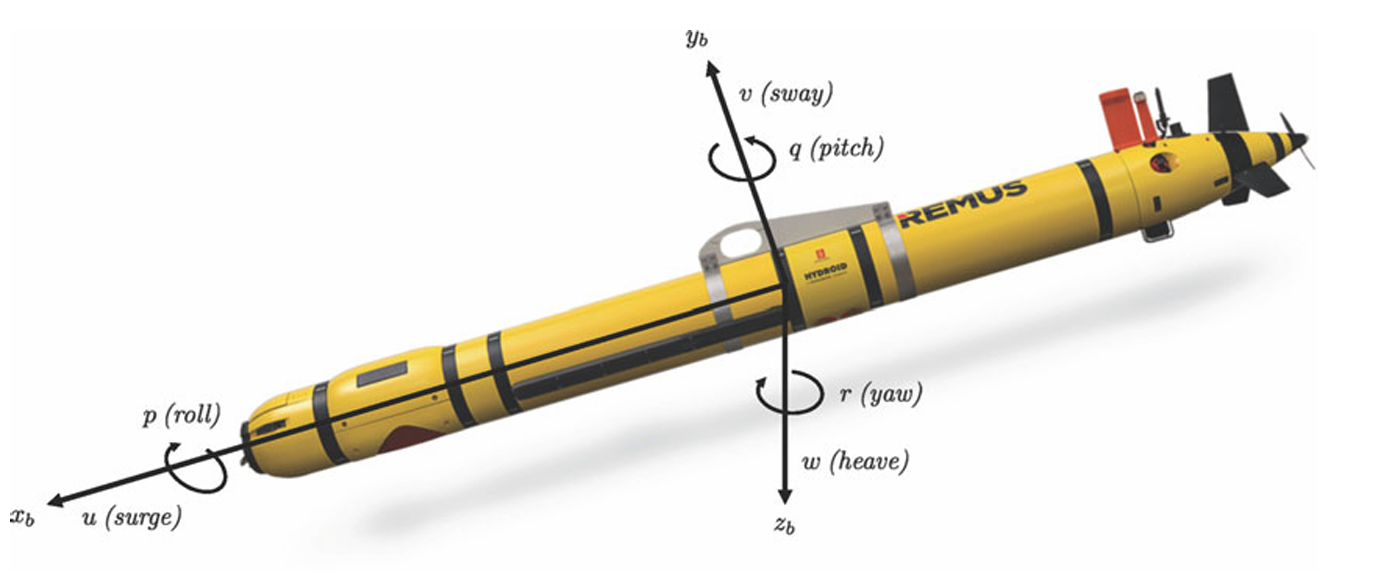
\includegraphics[width=0.7\linewidth]{img/6DOF motion AUV.png}};
	\end{tikzpicture}
	
	\vspace{2cm}
	
	Notation of SNAME (1950)
	\begin{itemize}
		\item Motion of $x$-direction (surge) -- $x$, controlled by $X$ [N]
		\item Motion of $y$-direction (sway) -- $y$, controlled by $Y$ [N]
		\item Motion of $z$-direction (heave) -- $z$, controlled by $Z$ [N]
		\item Rotation of $x$-direction (roll) -- $\phi$, controlled by $K$ [Nm]
		\item Rotation of $y$-direction (pitch) -- $\theta$, controlled by $M$ [Nm]
		\item Rotation of $z$-direction (yaw) -- $\psi$, controlled by $N$ [Nm]
	\end{itemize}
\end{frame}


% =========================================
% =========================================




\begin{frame}{Fundamental knowledge for modeling}
	\framesubtitle{General coordinates}
	
	\begin{tikzpicture}[remember picture,overlay]
		% \node[fill=blue!30, text=white, font=\large, rounded corners] 
		\node at (current page.north east) [xshift=-3.8cm, yshift=-3cm] 
		{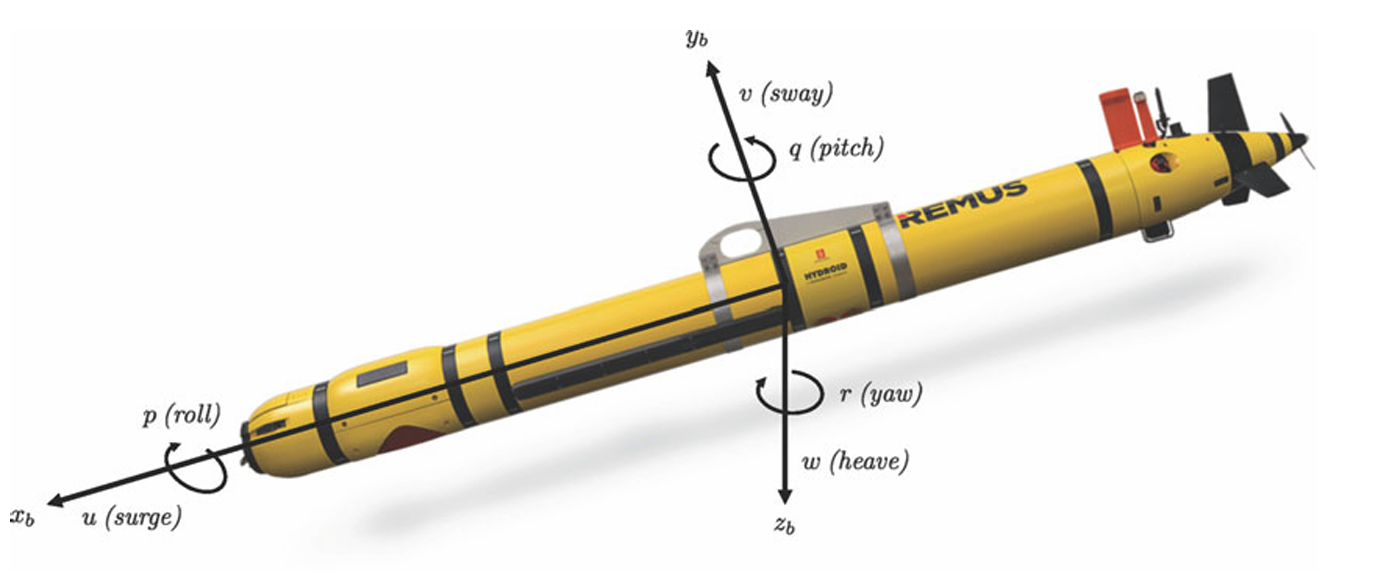
\includegraphics[width=0.7\linewidth]{img/6DOF motion AUV.png}};
	\end{tikzpicture}
	
	\vspace{2cm}
	
	
	General coordinate
	\begin{itemize}
		\item $\eta = \begin{bmatrix}
			(p_{b/n}^n)^\top & \Theta_{nb}^\top
		\end{bmatrix}^\top$, and $p_{b/n}^n = \begin{bmatrix}
			N & E & D
		\end{bmatrix}^\top$, $\Theta_{nb} = \begin{bmatrix}
			\phi & \theta & \psi
		\end{bmatrix}^\top$. In addition, the relative position of craft could be represented in frame ECI.
		\item $\nu = \begin{bmatrix}
			(v_{b/n}^b)^\top & (\omega_{b/n}^b)^\top
		\end{bmatrix}^\top$, and $v_{b/n}^b = \begin{bmatrix}
			u & v & w
		\end{bmatrix}^\top$, $\omega_{b/n}^b = \begin{bmatrix}
			p & q & r
		\end{bmatrix}^\top$
		\item $\tau = \begin{bmatrix}
			\tau_1^\top & \tau_2^\top
		\end{bmatrix}^\top$, and $\tau_1 = \begin{bmatrix}
			X & Y & Z
		\end{bmatrix}^\top$, $\tau_2 = \begin{bmatrix}
			K & M & N
		\end{bmatrix}^\top$
	\end{itemize}
	
	Notice that $\eta$ denotes the position and orientation vector with coordinates in the earth-fix frame. $\nu$ denotes the linear and angular velocity vector with coordinates in the body-fixed frame and $\tau$ denotes the force and torque acting on the vehicle.
	
	
\end{frame}


% =========================================
% =========================================


\begin{frame}{Fundamental knowledge for modeling}
	\framesubtitle{Euler angles}
	
	\begin{tikzpicture}[remember picture,overlay]
		\node at (current page.north east) [xshift=-3cm, yshift=-4.7cm] 
		{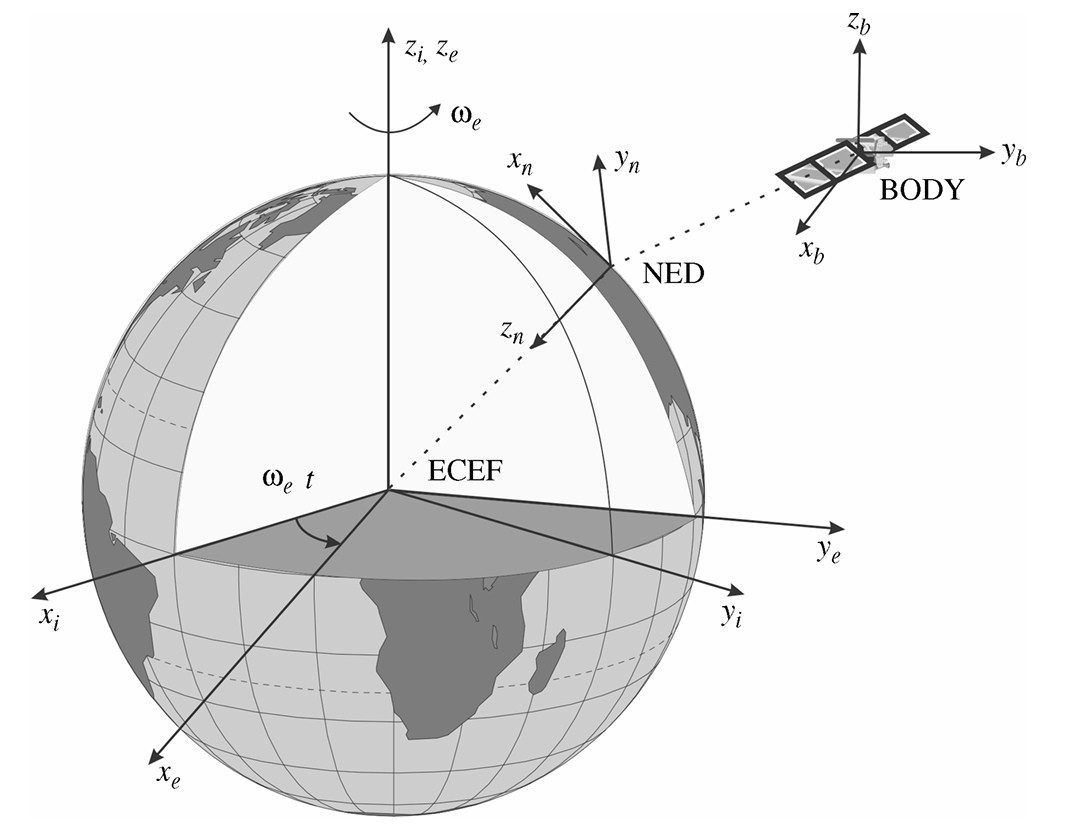
\includegraphics[width=0.5\linewidth]{img/frame.png}};
	\end{tikzpicture}
	
	Frames transformation
	\begin{itemize}
		\item Euler angles
		\item Rotation matrices
		\item Skew-Symmetric of a matrix
		\item Cross product
		\item Euler's theorem on rotation
		\item Linear/Angular velocity transformation
		\item Rotation matrix differential
		\item ...
	\end{itemize}
	
	\vspace{1cm}
	
	In another perspective, \textbf{quaternion} representation is also a good option!
\end{frame}



% =========================================
% =========================================


\begin{frame}{Fundamental knowledge for modeling}
	\framesubtitle{Kinematics}
	The 6 DOFs and 3 DOFs kinematic equations can be expressed in the following
	\begin{block}{6 DOFs kinematic equations}
		\begin{align}
			\dot{\eta} = J_{\Theta}(\eta)\nu
		\end{align}
		that is equivalent to
		\begin{align}
			\begin{bmatrix}
				\dot{p}_{b/n}^n \\ \dot{\Theta}_{nb}
			\end{bmatrix} = \begin{bmatrix}
				R_b^n & 0 \\
				0 & T_{\Theta}(\Theta_{nb})
			\end{bmatrix}\begin{bmatrix}
				v_{b/n}^b \\ \omega_{b/n}^b
			\end{bmatrix}
		\end{align}
		where $R_b^n$ and $T_{\Theta}(\Theta_{nb})$ denote the rotation and transformation matrices.
	\end{block}
	
	\begin{block}{3 DOFs kinematic equations}
		\begin{align}
			\dot{\eta} = R_z(\psi)\nu
		\end{align}
		with $\eta = \begin{bmatrix}
			x & y & \psi
		\end{bmatrix}^\top$ and $\nu = \begin{bmatrix}
			u & v & r
		\end{bmatrix}^\top$
	\end{block}
\end{frame}



% =========================================
% =========================================


\begin{frame}{Fundamental knowledge for modeling}
	\framesubtitle{Other transformations}
	
	In addition, for more purposes, other transformations are needed
	\begin{itemize}
		\item Transformation between ECEF and NED: wide area or terrestrial guidance and navigation.
		\item Transformation between BODY and FLOW: express the hydrodynamic data
	\end{itemize}
	\vspace{4cm}
	
	\begin{tikzpicture}[remember picture,overlay]
		% \node[fill=blue!30, text=white, font=\large, rounded corners] 
		\node at (current page.north west) [xshift=3cm, yshift=-6.5cm] {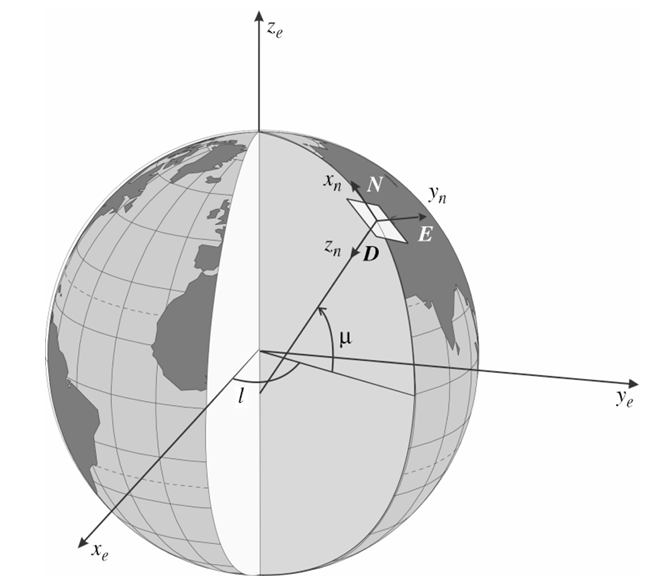
\includegraphics[width=0.4\linewidth]{img/earth surface.png}};
	\end{tikzpicture}
	
	\begin{tikzpicture}[remember picture,overlay]
		% \node[fill=blue!30, text=white, font=\large, rounded corners] 
		\node at (current page.north west) [xshift=8.5cm, yshift=-6.5cm] {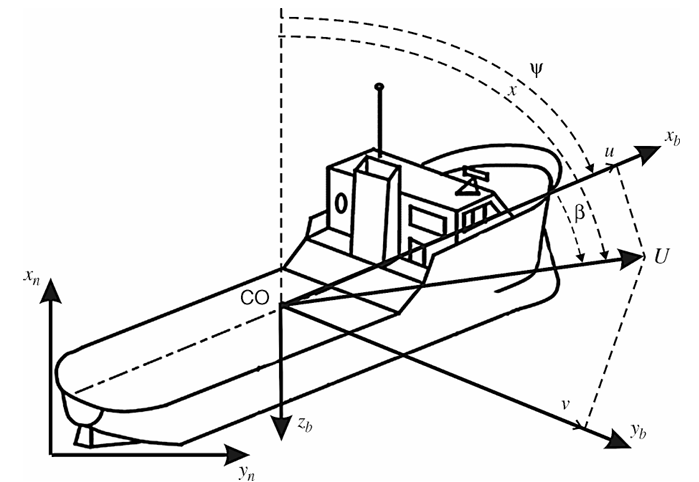
\includegraphics[width=0.5\linewidth]{img/geometrical relationship.png}};
	\end{tikzpicture}
\end{frame}


% =========================================
% =========================================


\begin{frame}{Fundamental knowledge for modeling}
	\framesubtitle{Transformation between BODY and FLOW}
	
	\begin{tikzpicture}[remember picture,overlay]
		% \node[fill=blue!30, text=white, font=\large, rounded corners] 
		\node at (current page.north east) [xshift=-3.8cm, yshift=-3.5cm] 
		{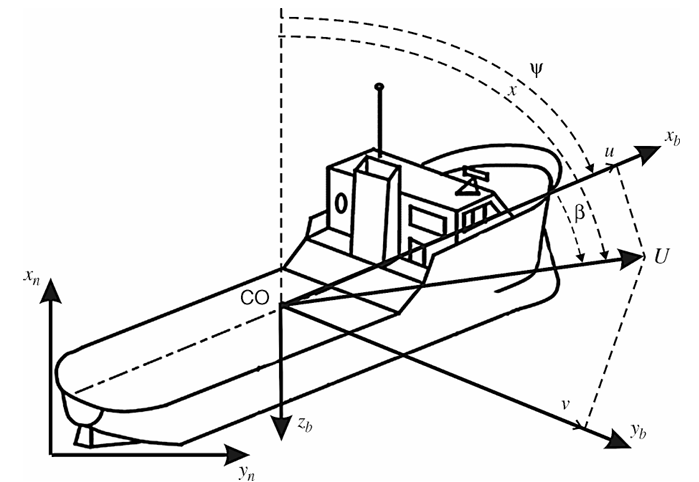
\includegraphics[width=0.5\linewidth]{img/geometrical relationship.png}};
	\end{tikzpicture}
	
	\vspace{1cm}
	
	Similarly, in the first case, the craft \\
	is assumed to be moving on the horizon.
	
	\vspace{0.5cm}
	
	Definition of Course, Heading,\\
	and Sideslip Angles
	\begin{itemize}
		\item Course angle $\chi$: The rotation of $x_n$ and \textbf{velocity vector} $u$ of craft around $z_n$
		\item Heading angle $\psi$: Yaw angle of craft
		\item Sideslip (Drift) angle $\beta$: The rotation of $x_b$ and \textbf{velocity vector} $u$ of craft around $z_b$
	\end{itemize}
	
	Thus $\chi = \psi + \beta$.
	
\end{frame}

% =========================================
% =========================================


\begin{frame}{Fundamental knowledge for modeling}
	\framesubtitle{Transformation between BODY and FLOW} \label{slide: Transformation between BODY and FLOW}
	\begin{tikzpicture}[remember picture,overlay]
		% \node[fill=blue!30, text=white, font=\large, rounded corners] 
		\node at (current page.north east) [xshift=-9.3cm, yshift=-4cm] 
		{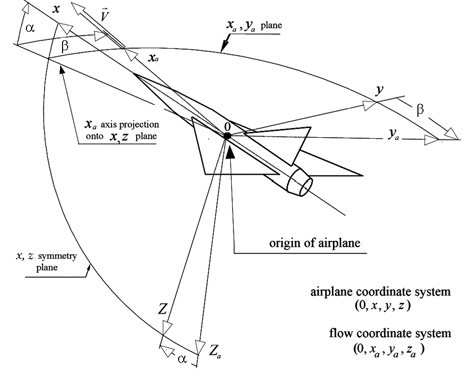
\includegraphics[width=0.55\linewidth]{img/sideslip.png}};
	\end{tikzpicture}
	
	
	\begin{tikzpicture}[remember picture,overlay]
		% \node[fill=blue!30, text=white, font=\large, rounded corners] 
		\node at (current page.north east) [xshift=-3cm, yshift=-3.5cm] 
		{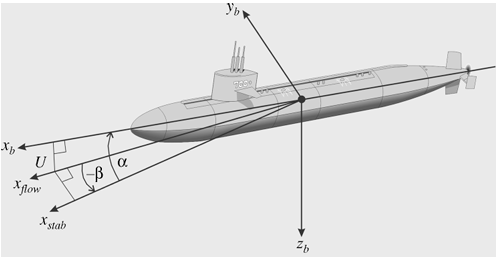
\includegraphics[width=0.5\linewidth]{img/flow UUV.png}};
	\end{tikzpicture}
	
	\vspace{4cm}
	
	\begin{block}{BODY to FLOW transformation}
		\begin{align}
			R_{b}^{flow} = R_{z, -\beta}R_{y, \alpha} = \begin{bmatrix}
				\cos\beta\cos\alpha & \sin\beta & \cos\beta\sin\alpha \\
				-\sin\beta \cos\alpha & \cos\beta & - \sin\beta\sin\alpha \\
				-\sin\alpha & 0 & \cos\alpha
			\end{bmatrix}
		\end{align}
	\end{block}
	
\end{frame}


% =========================================
% =========================================

\section{6-DOF model of a Rigid Body}
% =========================================
% =========================================


\begin{frame}{6-DOF model of a Rigid Body}
	\framesubtitle{Goal} 
	\begin{block}{Final goal}
		To find the equations that describe the behavior of the system
		\begin{align}
			M_{RB}\dot{\nu} + C_{RB}\nu = \tau_{RB}
		\end{align}
		in addition, as discussed above, 
		\begin{align}
			\dot{\eta} = J_{\Theta}(\eta)\nu
		\end{align}
	\end{block}
	\begin{itemize}
		\item Newton-Euler equations of motion about CG (Center gravity)
		\item Newton-Euler equations of motion about CO
	\end{itemize}
\end{frame}



% =========================================
% =========================================


\begin{frame}{6-DOF model of a Rigid Body}
	\framesubtitle{Fundamental}
	
	\begin{block}{Newton's second law}
		The Newton-Euler formulation is based on Newton's second law, which relates mass $m$, acceleration $\dot{\vec{v}}_{g/i}$ and force $\vec{f}_g$
		\begin{align}
			m\dot{\vec{v}}_{g/i} = \vec{f}_g
		\end{align}
	\end{block}
	
	\begin{block}{Euler's First and Second Axioms}
		The relationship between linear momentum and angular momentum
		\begin{align}
			\dfrac{d}{dt}\vec{p}_{g} = \vec{f}_g\\
			\dfrac{d}{dt}\vec{h}_{g} = \vec{m}_g
		\end{align}
		where $\vec{p}_{g}$ and $\vec{h}_{g}$ are the linear and angular momentum, respectively. $\vec{f}_g$ and $\vec{m}_g$ are the forces and moments acting on the CG.
	\end{block}
\end{frame}


% =========================================
% =========================================



\begin{frame}{6-DOF model of a Rigid Body}
	\framesubtitle{Fundamental}
	\begin{tikzpicture}[remember picture,overlay]
		% \node[fill=blue!30, text=white, font=\large, rounded corners] 
		\node at (current page.north east) [xshift=-3.8cm, yshift=-3.5cm] 
		{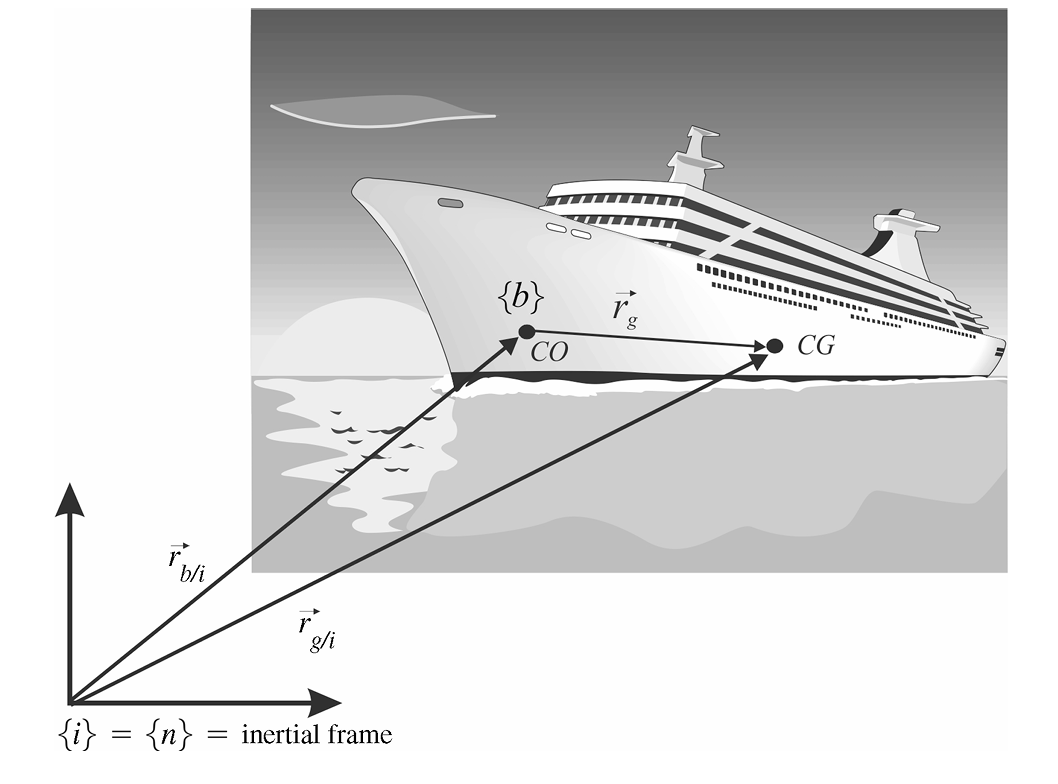
\includegraphics[width=0.5\linewidth]{img/coordinate.png}};
	\end{tikzpicture}
	
	\begin{itemize}
		\item Translational motion
		\item Rotational motion
	\end{itemize}
	
	\vspace{2cm}
	
	\begin{block}{Equations of Motion about CG}
		The Newton-Euler equation could be represented in the matrix form according to
		\begin{align}
			M_{RB}^{CG} \begin{bmatrix}
				\dot{v}_{g/n}^b \\ \dot{\omega}_{b/n}^b
			\end{bmatrix} + C_{RB}^{CG}\begin{bmatrix}
				{v}_{g/n}^b \\ {\omega}_{b/n}^b
			\end{bmatrix} = \begin{bmatrix}
				f_{g}^b \\ m_{g}^b
			\end{bmatrix}
		\end{align}
	\end{block}
\end{frame}

% =========================================
% =========================================

\begin{frame}{6-DOF model of a Rigid Body}
	\framesubtitle{Equations of Motion about CG}
	
	\begin{block}{Translational motion}
		Using Euler's first axiom,
		\begin{align}
			f_g = \dfrac{d}{dt}(mv_{g/i})
		\end{align}
		by several tedious mathematical transformations
		\begin{align}
			m\Big(\dot{v}_{g/n}^b + \omega_{b/n}^b\times v_{g/n}^b\Big) = f_{g}^b
		\end{align}
	\end{block}
	
	
	\begin{block}{Rotational motion}
		Using Euler's second axiom,
		\begin{align}
			m_g = \dfrac{d}{dt}(I_g\omega_{b/i})
		\end{align}
		by several tedious mathematical transformations
		\begin{align}
			I\dot{\omega}_{b/n}^{b} - S(I_g\omega_{b/n}^b) \times \omega_{b/n}^b = m_{g}^b
		\end{align}
	\end{block}
	
	
\end{frame}


% =========================================
% =========================================


\begin{frame}{6-DOF model of a Rigid Body}
	\framesubtitle{Equations of Motion about CO}
	By several SUPER TEDIOUS mathematical transformations
	\begin{block}{Nonlinear 6 DOF Rigid-Body Equations of Motion}
		\begin{align}
			m \big[\dot{u} - vr + wq - x_g(q^2 + r^2) + y_g(pq - \dot{r}) + z_g(pr + \dot{q})\big] = X, \\
			m \big[\dot{v} - wp + ur - y_g(r^2 + p^2) + z_g(qr - \dot{p}) + x_g(qp + \dot{r}) \big] = Y, \\
			m \big[\dot{w} - uq + vp - z_g(p^2 + q^2) + x_g(rp - \dot{q}) + y_g(r \dot{p})\big] = Z,
			\\
			I_x \dot{p} + (I_z - I_y)qr - (r + pq)I_{xz} + (r^2 - q^2)I_{yz} + (pr - \dot{q})I_{xy} & \notag\\
			+ m \big[ y_g(\dot{w} - uq + vp) - z_g(\dot{v} - wp + ur) )= K, \\
			I_y \dot{q} + (I_x - I_z)rp - (p + qr)I_{xy} + (p^2 - r^2)I_{zx} + (qp - \dot{r})I_{yz} & \notag \\
			+ m \big[ z_g(\dot{u} - vr + wq) - x_g(\dot{w} - uq + vp) ) = M, \\
			I_z \dot{r} + (I_y - I_x)pq - (q + rp)I_{xz} + (q^2 - p^2)I_{xx} + (rq - \dot{p})I_{zx} & \notag \\
			+ m \big[ x_g(\dot{v} - wp + ur) - y_g(\dot{u} - vr + wq)) = N.
		\end{align}
	\end{block}
\end{frame}

% =========================================
% =========================================



\begin{frame}{6-DOF model of a Rigid Body}
	\framesubtitle{Matrix Form}
	\begin{block}{Rigid-body dynamics model}
		\begin{align}
			M_{RB}\dot{\nu} + C_{RB}\nu = \tau_{RB}
		\end{align}
		where
		\begin{align}
			M_{RB} = \begin{bmatrix}
				mI_{3\times 3} & -mS(r_g^b) \\
				mS(r_g^b) & I_b
			\end{bmatrix} \\
			C_{RB} = \begin{bmatrix}
				0_{3\times 3} & -S(M_{11}\nu_1 + M_{12}\nu_2) \\
				-S(M_{11}\nu_1 + M_{12}\nu_2) & -S(M_{21}\nu_1 + M_{22}\nu_2)
			\end{bmatrix} 
		\end{align}
	\end{block}
\end{frame}



% =========================================
% =========================================




\begin{frame}{6-DOF model of a Rigid Body}
	\framesubtitle{Linearized 6 DOF Rigid body Equation of Motion}
	
	
\end{frame}
% =========================================
% =========================================




\begin{frame}{Dynamics model}
	\framesubtitle{Simplifyed 6 DOF Rigid body Equation of Motion}
	\begin{itemize}
		\item The Origin CO coincides with the CG
		\item Translation of the origin CO such that $I_b$ becomes diagonal
	\end{itemize}
	\begin{block}{Simplifyed 6 DOF Rigid body Equation of Motion}
		\begin{align}
			m \big[ \dot{u} - vr + wq - x_g (q^2 + r^2) + y_g (pq - \dot{r}) + z_g (pr + \dot{q}) \big] &= X, \\
			m \big[ \dot{v} - wp + ur - y_g (r^2 + p^2) + z_g (qr - \dot{p}) + x_g (qp + \dot{r}) \big] &= Y, \\
			m \big[ \dot{w} - uq + vp - z_g (p^2 + q^2) + x_g (rp - \dot{q}) + y_g (rq + \dot{p}) \big] &= Z, \\
			I_x \dot{p} + (I_z - I_y) qr + m \big[ y_g (\dot{w} - uq + vp) - z_g (\dot{v} - wp + ur) \big] &= K, \\
			I_y \dot{q} + (I_x - I_z) rp + m \big[ z_g (\dot{u} - vr + wq) - x_g (\dot{w} - uq + vp) \big] &= M, \\
			I_z \dot{r} + (I_y - I_x) pq + m \big[ x_g (\dot{v} - wp + ur) - y_g (\dot{u} - vr + wq) \big] &= N.
		\end{align}
	\end{block}
\end{frame}


% =========================================
% =========================================

\section{Ocean dynamics}
% =========================================
% =========================================




\begin{frame}{Ocean dynamics}
	\framesubtitle{Hydrostatics}
	\begin{tikzpicture}[remember picture,overlay]
		% \node[fill=blue!30, text=white, font=\large, rounded corners] 
		\node at (current page.north east) [xshift=-3.8cm, yshift=-3cm] 
		{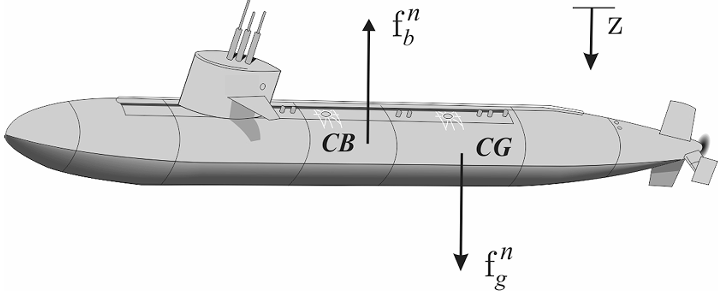
\includegraphics[width=0.7\linewidth]{img/force.png}};
	\end{tikzpicture}
	
	\vspace{1cm}
	
	Forces act in the vertical plane 
	\begin{align}
		f_g^n = \begin{bmatrix}
			0 & 0 & W
		\end{bmatrix}^\top; \quad f_b^n = -\begin{bmatrix}
			0 & 0 & B
		\end{bmatrix}^\top
	\end{align}
	Thus, the gravity vector is
	\begin{align}
		{g}(\eta) &= - 
		\begin{bmatrix}
			{f}_g^b + {f}_b^b \\
			{r}_g^b \times {f}_g^b + {r}_b^b \times {f}_b^b
		\end{bmatrix} \\
		&= - 
		\begin{bmatrix}
			{R}_b^n (\Theta_{nb})^{-1} \left( {f}_g^n + {f}_b^n \right) \\
			{r}_g^b \times {R}_b^n (\Theta_{nb})^{-1} {f}_g^n + 
			{r}_b^b \times {R}_b^n (\Theta_{nb})^{-1} {f}_b^n
		\end{bmatrix}.
	\end{align}
	\textbf{Note:} These formulations become more complex when considering the surface vessels
\end{frame}



% =========================================
% =========================================



\begin{frame}{Ocean dynamics}
	\framesubtitle{Seakeeping Theory(wave and wind)}
	\begin{block}{Vehicle-Ocean dynamics model}
		\begin{align}
			\dot{\eta} = J_{\Theta}(\eta)\nu \notag \\
			M_{RB} \dot{\nu} + C_{RB}^* \nu + M_A \dot{\nu}_r + C_A^* \nu_r + (D_P + D_V) \nu_r + \mu + G \eta + g_o = \tau_{\text{wind}} + \tau_{\text{wave}}  + \tau  \notag
		\end{align}
	\end{block}
	\begin{block}{Vehicle-Ocean dynamics model}
		\begin{align}
			\text{Inertia forces:} & \quad M_{RB} \dot{\nu} + C_{RB}^* \nu + M_A \dot{\nu}_r + C_A^* \nu_r \notag\\
			\text{Damping forces:} & \hspace{1.8cm} + (D_P + D_V) \nu_r + \mu \notag\\
			\text{Restoring forces:} & \hspace{3.3cm} + G \eta + g_o \notag\\
			\text{Wind and wave forces:} & \hspace{5cm} = \tau_{\text{wind}} + \tau_{\text{wave}} \notag\\
			\text{Propulsion forces:} & \hspace{5.5cm} + \tau \notag
		\end{align}
	\end{block}
\end{frame}

% =========================================
% =========================================


\begin{frame}{Ocean dynamics}
	\framesubtitle{Seakeeping kinematics (wave and wind)}
	\begin{tikzpicture}[remember picture,overlay]
		% \node[fill=blue!30, text=white, font=\large, rounded corners] 
		\node at (current page.north east) [xshift=-4cm, yshift=-4cm] 
		{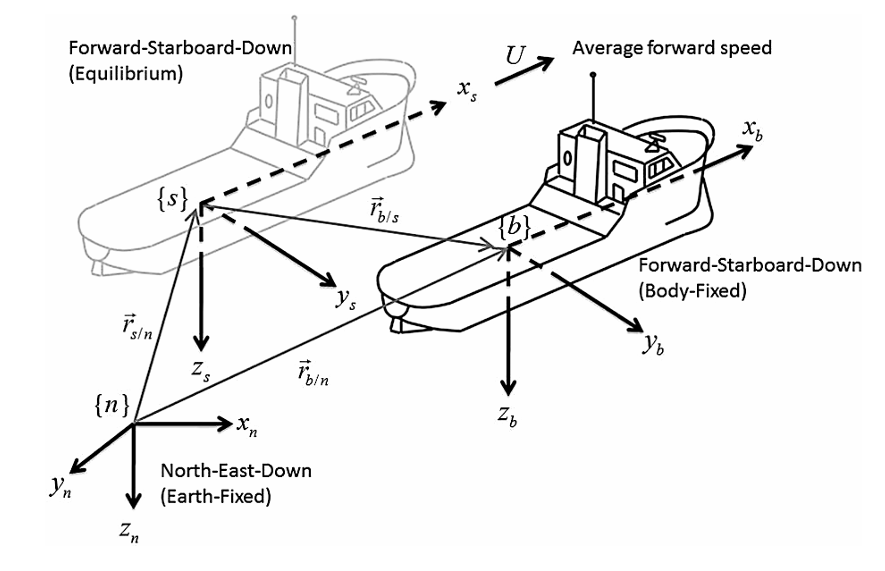
\includegraphics[width=0.7\linewidth]{img/seakeeping.png}};
	\end{tikzpicture}
	
	\vspace{4cm}
	
	Several notations
	\begin{itemize}
		\item $v_{s/n}^n = \begin{bmatrix}
			U\cos{\bar{\psi}} & U\sin{\bar{\psi}} & 0
		\end{bmatrix}^\top$
		\item $\omega_{s/n}^n = \begin{bmatrix}
			0 & 0 & 0
		\end{bmatrix}^\top$
		\item $\Theta_{ns} = \begin{bmatrix}
			0 & 0 & \bar{\psi}
		\end{bmatrix}^\top$
	\end{itemize}
	
\end{frame}


% =========================================
% =========================================


\begin{frame}{Ocean dynamics}
	\framesubtitle{Seakeeping kinematics(wave and wind)}
	Define the perturbation coordinate
	\begin{align}
		\delta\eta = \begin{bmatrix}
			r_{b/s}^s \\ \Theta_{sb}
		\end{bmatrix}; \quad \delta \nu = \begin{bmatrix}
			v_{b/s}^b \\ \omega_{b/s}^b
		\end{bmatrix} ; \quad \xi = \delta \eta; \quad \Theta_{sb} = \begin{bmatrix}
			\delta\phi \\ \delta\theta \\ \delta\psi
		\end{bmatrix}
	\end{align}
	Thus, the following equations are achieved as the transformation between BODY and SEAKEEPING coordinates
	\begin{block}{Transformation between BODY and SEAKEEPING}
		\begin{align}
			\dot{\nu} = -UL\delta\nu + \delta\dot{\nu}
		\end{align}
		where $U$ is the velocity of the vehicle and $L \in \mathbb{R}_{6\times 6}$\\
		\textbf{Linear transformations}
		\begin{align}
			\delta\nu \approx \nu + U(L\delta\eta - e_1)\\
			\delta\dot{\nu} \approx \dot{\nu} + UL\nu
		\end{align}
	\end{block}
\end{frame}



% =========================================
% =========================================



\begin{frame}{Ocean dynamics}
	\framesubtitle{Added mass(wave and wind)}
	From Cummins Equation in SEAKEEPING Coordinates, the following equations are introduced
	\begin{block}{Frequency-domain seakeeping equation of motion}
		\begin{align}
			\Big(-\omega^2(M_{RB} + \bar{A}(\omega
			)) - j\omega B(\omega) + C
			\Big)\ddot{\xi}(j\omega
			)= \tau_{wind}(j\omega)+ \tau_{wave}(j\omega) + \delta\tau(j\omega)
		\end{align}
	\end{block}
	
	\begin{block}{Time-domain seakeeping equation of motion}
		\begin{align}
			\Big(M_{RB} + \bar{A}\Big)\ddot{\xi} + \int\limits_{-\infty}^t \bar{K}(t - \tau)\dot{\xi}(t)d\tau + \bar{C}\xi = \tau_{wind} + \tau_{wave} + \delta\tau
		\end{align}
	\end{block}
	where $\bar{K} = \dfrac{2}{\pi}\int\limits_{0}^{\infty}B(\omega)\cos(\omega t)d\omega$
	
	\textbf{Notice:} For underwater vehicle, $A(\omega) = \text{const}$ and $B(\omega) = 0$
\end{frame}



% =========================================
% =========================================


\begin{frame}{Ocean dynamics}
	\framesubtitle{Added mass(wave and wind)}
	\begin{block}{Hydrodynamic added mass forces and moments in 6 DOFs}
		\begin{itemize}
			\item The expressions are complicated and not suited for control design.
			\item Hydrodynamic software programs such as WAMIT and ShipX can be used to compute the added mass term.
		\end{itemize}
	\end{block}
	\vspace{4cm}
	
	\begin{tikzpicture}[remember picture,overlay]
		% \node[fill=blue!30, text=white, font=\large, rounded corners] 
		\node at (current page.north west) [xshift=3cm, yshift=-6.5cm] {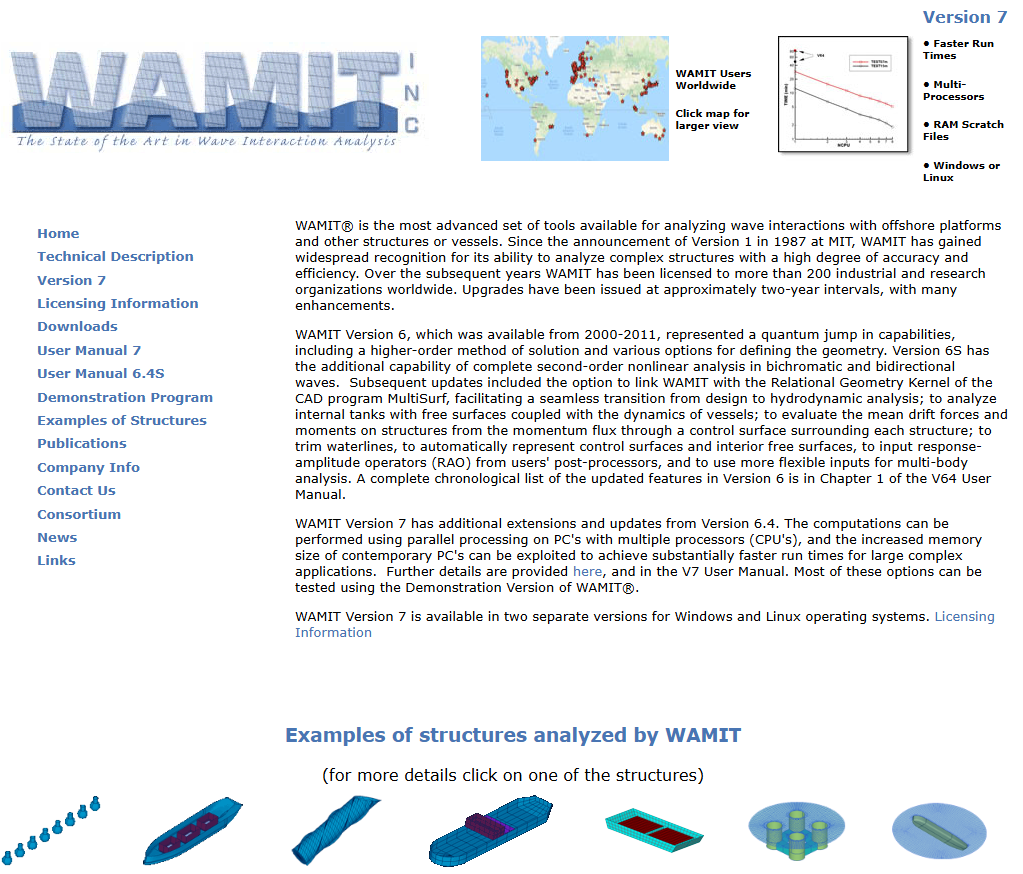
\includegraphics[width=0.4\linewidth]{img/wamit.png}};
	\end{tikzpicture}
	
	\begin{tikzpicture}[remember picture,overlay]
		% \node[fill=blue!30, text=white, font=\large, rounded corners] 
		\node at (current page.north west) [xshift=9.5cm, yshift=-6.5cm] {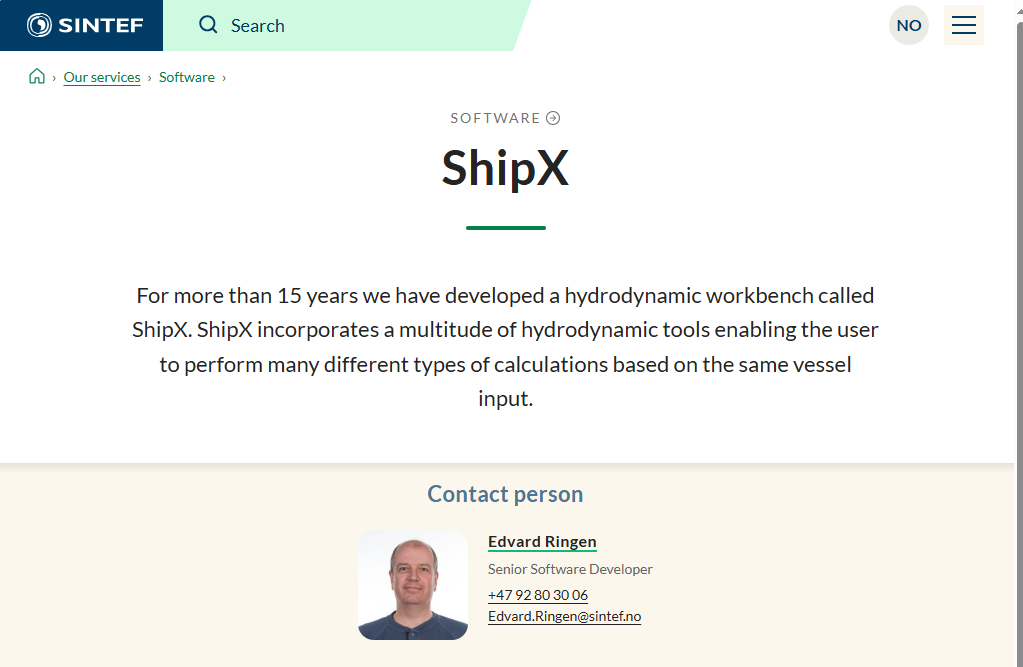
\includegraphics[width=0.5\linewidth]{img/shipX.png}};
	\end{tikzpicture}
\end{frame}


% =========================================
% =========================================


\begin{frame}{Ocean dynamics}
	\framesubtitle{Linear equation of motion}
	From Cummins Equation in SEAKEEPING Coordinates, the following equations are introduced
	\begin{block}{Linear equation of motion (Zero-Speed Potential Coefficients)}
		\begin{align}
			M\dot{\nu} + C_{RB}^*\nu + C_A^*\nu_r + D\nu_r + \int\limits_0^tK(t-\tau)[\nu(\tau) - Ue_1]d\tau + G\eta = \sum\tau
		\end{align}
	\end{block}
	\begin{block}{Linear equation of motion (Speed-Dependent Potential Coefficients)}
		\begin{align}
			M_U\dot{\nu} + C_{RB}^*\nu + C_A^*\nu_r + D_U\nu_r + \int\limits_0^tK_U(t-\tau)[\nu(\tau) - Ue_1]d\tau + G\eta = \sum\tau
		\end{align}
	\end{block}
	where $\sum\tau = \tau_{wind} + \tau_{wind} + \tau$
\end{frame}


% =========================================
% =========================================


\begin{frame}{Ocean dynamics}
	\framesubtitle{Maneuvering Theory}
	\begin{block}{Goal}
		\begin{align}
			\underbrace{{M_{RB} \dot{\nu} + C_{RB}(\nu) \nu}}_{\text{rigid-body forces}} + 
			\underbrace{{M_A \dot{\nu}_r + C_A(\nu_r) \nu_r + D(\nu_r) \nu_r}}_{\text{hydrodynamic forces}}
			+\underbrace{{g(\eta) + g_o}}_{\text{hydrostatic forces}}
			= \tau + \tau_{\text{wind}} + \tau_{\text{wave}}
		\end{align}
		or
		\begin{align}
			M \dot{\nu}_r + C(\nu_r) \nu_r + D(\nu_r) \nu_r + g(\eta) + g_o = \tau + \tau_{\text{wind}} + \tau_{\text{wave}}
		\end{align}
		where $\nu_r = \nu - \nu_c$ is the relative velocity vector.
	\end{block}
	\begin{itemize}
		\item For slender bodies, such as AUV, the longitudinal (surge, heave, and pitch motion) and lateral (sway, roll, and yaw motion) models are referred to consider.
		\item For ROVs operating, the horizontal-plane (surge, sway, and yaw motion) and depth (heavy) models are referred to consider.
	\end{itemize}
\end{frame}




% =========================================
% =========================================


\begin{frame}{Ocean dynamics}
	\framesubtitle{Maneuvering Theory - 3DOF maneuvering model}
	\begin{block}{3DOF maneuvering model}
		The horizontal motions (surge, sway, and heave) of a marine craft moving at forward speed could be described by a zero frequency model, where
		\begin{align}
			M_A = \begin{bmatrix}
				A_{11}(0) & 0 & 0 \\
				0 & A_{22}(0) & A_{26}(0) \\
				0 & A_{62}(0) & A_{66}(0)
			\end{bmatrix}\\
			D_p = 0
		\end{align}
		are the constant matrices.
	\end{block}
	\textbf{Limitation}  One limitation of the zero-frequency assumption is that it cannot be applied to heave, roll, and pitch.  For 2nd-order mass-damper-spring systems the dominating frequencies are the natural frequencies.
\end{frame}


% =========================================
% =========================================


\begin{frame}{Ocean dynamics}
	\framesubtitle{Extension to 6-DOF models}
	\begin{block}{Extension to 6-DOF models}
		\textbf{Solution:} Formulate frequency-independent models in heave, pitch, and roll at their respective natural frequencies and not the zero frequency.
		\begin{align}
			\omega_3 = \sqrt{\dfrac{C_{33}}{m + A_{33}(\omega_3)}}\\
			\omega_4 = \sqrt{\dfrac{C_{44}}{I_x + A_{44}(\omega_4)}}\\
			\omega_5 = \sqrt{\dfrac{C_{55}}{I_y + A_{55}(\omega_5)}}
		\end{align}
	\end{block}
	\textbf{Key assumption:} No coupling between the surge-sway-yaw and the heave-roll-pitch subsystems.
\end{frame}



% =========================================
% =========================================


\begin{frame}{Ocean dynamics}
	\framesubtitle{Added Mass Forces in a Rotating Coordinate System}
	The expression for the fluid kinetic energy \( T_A \), see Ref. \footnote{Imlay, Frederick H. \textit{The complete expressions for added mass of a rigid body moving in an ideal fluid}. No. Report 1528. 1961.}, can be written as a quadratic form of the body axis velocity vector components, that is:
	\begin{align}
		T_A = \frac{1}{2} \boldsymbol{\nu}^T M_A \boldsymbol{\nu}
	\end{align}
	
	Here \( M_A \) is a \( 6 \times 6 \) added inertia matrix defined as:
	\begin{align}
		M_A = 
		\begin{bmatrix}
			A_{11} & A_{12} \\
			A_{21} & A_{22}
		\end{bmatrix}
		\triangleq - 
		\begin{bmatrix}
			X_{\dot{u}} & X_{\dot{v}} & X_{\dot{w}} & X_{\dot{p}} & X_{\dot{q}} & X_{\dot{r}} \\
			Y_{\dot{u}} & Y_{\dot{v}} & Y_{\dot{w}} & Y_{\dot{p}} & Y_{\dot{q}} & Y_{\dot{r}} \\
			Z_{\dot{u}} & Z_{\dot{v}} & Z_{\dot{w}} & Z_{\dot{p}} & Z_{\dot{q}} & Z_{\dot{r}} \\
			K_{\dot{u}} & K_{\dot{v}} & K_{\dot{w}} & K_{\dot{p}} & K_{\dot{q}} & K_{\dot{r}} \\
			M_{\dot{u}} & M_{\dot{v}} & M_{\dot{w}} & M_{\dot{p}} & M_{\dot{q}} & M_{\dot{r}} \\
			N_{\dot{u}} & N_{\dot{v}} & N_{\dot{w}} & N_{\dot{p}} & N_{\dot{q}} & N_{\dot{r}}
		\end{bmatrix}, \quad Y_A = Y_{\dot{u}}\dot{u}, \quad Y_{\dot{u}} \triangleq \dfrac{\partial Y}{\partial \dot{u}}
	\end{align}
	\textbf{Notice:} In a real fluid, these 36 constants could be distinct. With ideal (without friction),$M_A = M_A^\top$
\end{frame}



% =========================================
% =========================================


\begin{frame}{Ocean dynamics}
	\framesubtitle{Added Mass Forces in a Rotating Coordinate System}
	\begin{block}{Hydrodynamic Coriolis-Centripetal Matrix $C_A(\nu)$}
		For a rigid body moving through an ideal fluid the hydrodynamic Coriolis and centripetal matrix $C_A(\nu)$ could always be parametrized such that it is skew-symmetric
		\begin{align}
			C_A(\nu) = -C_A(\nu)^\top, \quad \forall\nu
		\end{align}
		As mentioned above,
		\begin{align}
			C_A(\nu) = \begin{bmatrix}
				0 & -S(A_{11}\nu_1 + A_{12}\nu_2) \\
				-S(A_{11}\nu_1 + A_{12}\nu_2) & -S(A_{21}\nu_1 + A_{22}\nu_2) 
			\end{bmatrix}
		\end{align}
	\end{block}
\end{frame}

% =========================================
% =========================================



\begin{frame}{Ocean dynamics}
	\framesubtitle{Added Mass Forces in a Rotating Coordinate System}
	\begin{block}{Vehicle-Ocean dynamics model}
		\begin{align}
			\dot{\eta} = J_{\Theta}(\eta)\nu \notag \\
			M_{RB} \dot{\nu} + C_{RB}^* \nu + M_A \dot{\nu}_r + C_A^* \nu_r + (D_P + D_V) \nu_r + \mu + G \eta + g_o = \tau_{\text{wind}} + \tau_{\text{wave}}  + \tau  \notag
		\end{align}
	\end{block}
	\begin{block}{Vehicle-Ocean dynamics model}
		\begin{align}
			\text{Inertia forces:} & \quad M_{RB} \dot{\nu} + C_{RB}^* \nu + M_A \dot{\nu}_r + C_A^* \nu_r \notag\\
			\text{Damping forces:} & \hspace{1.8cm} + (D_P + D_V) \nu_r + \mu \notag\\
			\text{Restoring forces:} & \hspace{3.3cm} + G \eta + g_o \notag\\
			\text{Wind and wave forces:} & \hspace{5cm} = \tau_{\text{wind}} + \tau_{\text{wave}} \notag\\
			\text{Propulsion forces:} & \hspace{5.5cm} + \tau \notag
		\end{align}
	\end{block}
\end{frame}




% =========================================
% =========================================




\begin{frame}{Ocean dynamics}
	\framesubtitle{Viscous damping}
	In practical implementations, it is difficult to determine higher-order terms as well as the off-diagonal terms in general expression for hydrodynamic damping.
	
	The different damping terms contribute to both linear and quadratic damping. However, it is in general difficult to separate these effects. In many cases, it is convenient to write total hydrodynamic damping as
	\begin{align}
		D(\nu_r) = D + D_n(\nu_r)
	\end{align}
	\begin{itemize}
		\item Linear viscous damping
		\begin{align}
			D = D_p + D_v \approx -diag(X_u, Y_v, Z_w, K_p, M_q, N_r)
		\end{align}
		\item Nonlinear surge damping
		\begin{itemize}
			\item Nonlinear Surge Damping: Damping Due to Vortex Shedding
			\item Cross-Flow Drag Principle (lifting Forces:): For relative current angles, the cross-flow drag principle may be applied to calculate the nonlinear damping force in sway and the yaw moment
		\end{itemize}
	\end{itemize}
\end{frame}






% =========================================
% =========================================




\begin{frame}{Ocean dynamics}
	\framesubtitle{Linear viscous damping}
	The approximate diagonal matrix $D_p$ is expressed as:
	
	\begin{equation}
		D_p \approx 
		\begin{bmatrix}
			0 & 0 & 0 & 0 & 0 & 0 \\
			0 & 0 & 0 & 0 & 0 & 0 \\
			0 & 0 & B_{33}(\omega_\text{heave}) & 0 & 0 & 0 \\
			0 & 0 & 0 & B_{44}(\omega_\text{roll}) & 0 & 0 \\
			0 & 0 & 0 & 0 & B_{55}(\omega_\text{pitch}) & 0 \\
			0 & 0 & 0 & 0 & 0 & 0
		\end{bmatrix} 
	\end{equation}
	
	The natural frequencies $\omega_\text{heave}$, $\omega_\text{roll}$, and $\omega_\text{pitch}$ can be computed as introduced in the above.
	
	A diagonal matrix usually approximates the linear viscous damping terms:
	\begin{equation}
		D_v \approx \text{diag}\{B_{11v}, B_{22v}, B_{33v}, B_{44v}, B_{55v}, B_{66v}\}
	\end{equation}
	
	where the elements $B_{iiv} \; (i = 1, \ldots, 6)$ can be computed from the time constants and natural periods of the system (see Section 6.4).
\end{frame}




% =========================================
% =========================================



\begin{frame}{Ocean dynamics}
	\framesubtitle{Linear viscous damping}
	The expressions for the diagonal elements of $D_v$ are as follows:
	\begin{align}
		B_{11v} &= \frac{m + A_{11}(0)}{T_\text{surge}} = \frac{8\pi \zeta_\text{surge}[m + A_{11}(0)]}{T_{n,\text{surge}}} \\
		B_{22v} &= \frac{m + A_{22}(0)}{T_\text{sway}} = \frac{8\pi \zeta_\text{sway}[m + A_{22}(0)]}{T_{n,\text{sway}}} \\
		B_{33v} &= 2\Delta \zeta_\text{heave} \omega_\text{heave} [m + A_{33}(\omega_\text{heave})] \\
		B_{44v} &= 2\Delta \zeta_\text{roll} \omega_\text{roll} [I_x + A_{44}(\omega_\text{roll})] \\
		B_{55v} &= 2\Delta \zeta_\text{pitch} \omega_\text{pitch} [I_y + A_{55}(\omega_\text{pitch})] \\
		B_{66v} &= \frac{I_z + A_{66}(0)}{T_\text{yaw}} = \frac{8\pi \zeta_\text{yaw}[I_z + A_{66}(0)]}{T_{n,\text{yaw}}}
	\end{align}
\end{frame}




% =========================================
% =========================================





\begin{frame}{Ocean dynamics}
	\framesubtitle{Nonlinear viscous damping}
	\begin{block}{Quadratic drag and lifting in 6DOF}
		Quadratic drag and lifting in 6DOF
		\begin{align}
			D_n(\nu_r)\nu_r = [|\nu_r|^\top D_i(\rho, A, C_D)\nu_r)]_{6\times1}
		\end{align}
		The viscous damping force due to vortex shedding can be modeled as
		\begin{align}
			f(U) = -\dfrac{1}{2}\rho C_D A |U_r|U_r
		\end{align}
		where $\rho$ is the fluid density, $C_D$ is drag coefficient, $A$ is the projected cross-sectional area, and $U$ is the velocity of the vehicle.
	\end{block}
\end{frame}




% =========================================
% =========================================



\begin{frame}{Ocean dynamics}
	\framesubtitle{Maneuvering Equations}
	
	\textbf{{Hydrodynamic Mass--Damper}}
	
	\begin{itemize}
		\item \textbf{Added mass} $M_A$ due to the inertia of the surrounding fluid (see Section 6.2). The corresponding Coriolis and centripetal matrix due to added mass is due to the rotation of $\{b\}$ with respect to $\{n\}$ and is denoted $C_A({v}_r)$ (see Section 6.3).
		\item \textbf{Radiation-induced potential damping} $D_p$ due to the energy carried away by generated surface waves.
		\item \textbf{Viscous damping} caused by skin friction, wave drift damping, vortex shedding, and lift/drag (see Section 6.4). 
	\end{itemize}
	The resulting hydrodynamic force is written as:
	\begin{align}
		{\tau}_\text{hyd} = -M_A \dot{\nu}_r - C_A(\nu_r) \nu_r - D_p \nu_r + {\tau}_\text{visc}
	\end{align}
	where $\nu_r = \nu - \nu_c$ with $\nu_c = [u_c, v_c, w_c, 0, 0, 0]^\top$ is the relative velocity due to an \textit{irrotational constant ocean current} (see Section 8.3), and
	\begin{align}
		{\tau}_\text{visc} = -D_v {v}_r - D_n({v}_r) {v}_r
	\end{align}
	\textbf{{Hydrostatic Spring Stiffness}}: \textbf{Restoring forces} due to Archimedes
	\begin{align}
		{\tau}_\text{hs} = -g({\eta}) - {g}_o
	\end{align}
\end{frame}


% =========================================
% =========================================



\section{Environmental Disturbances}
% =========================================
% =========================================

\begin{frame}{Environmental Disturbances}
	The environmental disturbances include
	\begin{itemize}
		\item Wind forces and moments
		\item Wave forces and moments
	\end{itemize}
	
	In this context, if the autonomous underwater vehicles are considered to be working at the deep water level, the wind and wave disturbances are not significant enough to be considered.
	
	\vspace{1cm}
	The wind and wave disturbances become more significant when we consider a surface vehicle, and it could be introduced in the future version.
	
	
	[Coming soon!!]
\end{frame}



\section{An example of the ODIN}

\begin{frame}{An example of the ODIN}
	\framesubtitle{Rigid body equation of motion}
	ODIN = Omni-directional intelligent navigation \footnote{Choi, Hyun-Taek, et al. "Development of an underwater robot, ODIN-III." Proceedings 2003 IEEE/RSJ International Conference on Intelligent Robots and Systems (IROS 2003)(Cat. No. 03CH37453). Vol. 1. IEEE, 2003.},\footnote{Ali, Nihad, Isaac Tawiah, and Weidong Zhang. "Finite-time extended state observer based nonsingular fast terminal sliding mode control of autonomous underwater vehicles." Ocean Engineering 218 (2020): 108179.}
	
	\begin{tikzpicture}[remember picture,overlay]
		% \node[fill=blue!30, text=white, font=\large, rounded corners] 
		\node at (current page.north east) [xshift=-3cm, yshift=-5.5cm] 
		{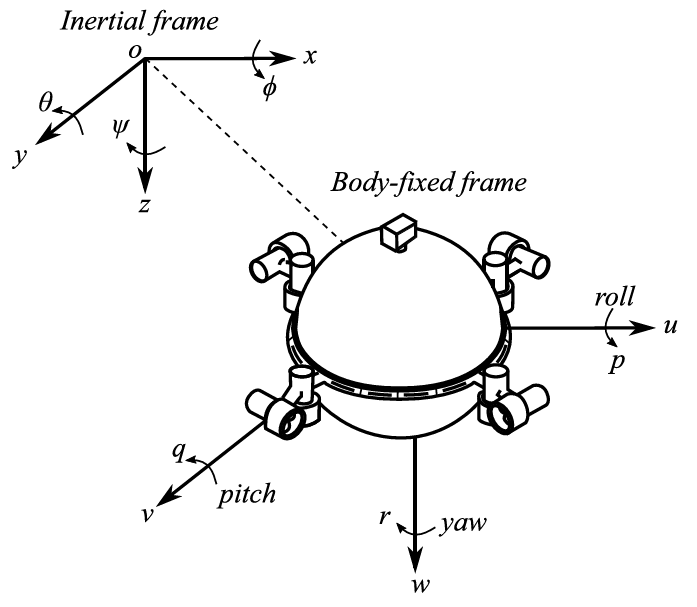
\includegraphics[width=0.4\linewidth]{img/ODIN.png}};
	\end{tikzpicture}
	
	\begin{tikzpicture}[remember picture,overlay]
		% \node[fill=blue!30, text=white, font=\large, rounded corners] 
		\node at (current page.north east) [xshift=-7cm, yshift=-5.5cm] 
		{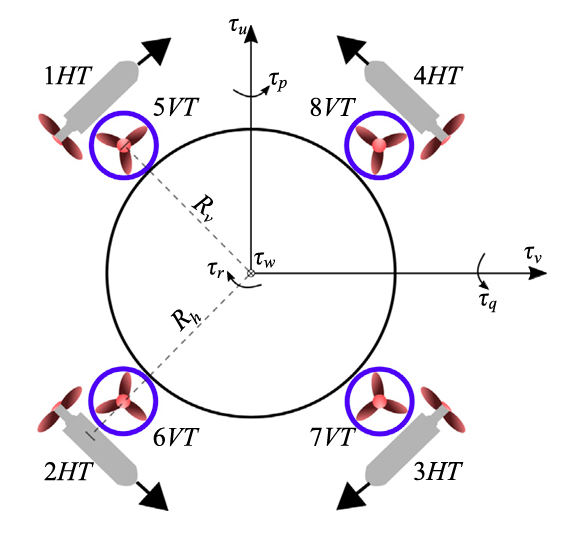
\includegraphics[width=0.25\linewidth]{img/ODIN1.png}};
	\end{tikzpicture}
	
	\begin{tikzpicture}[remember picture,overlay]
		% \node[fill=blue!30, text=white, font=\large, rounded corners] 
		\node at (current page.north east) [xshift=-11cm, yshift=-5.5cm] 
		{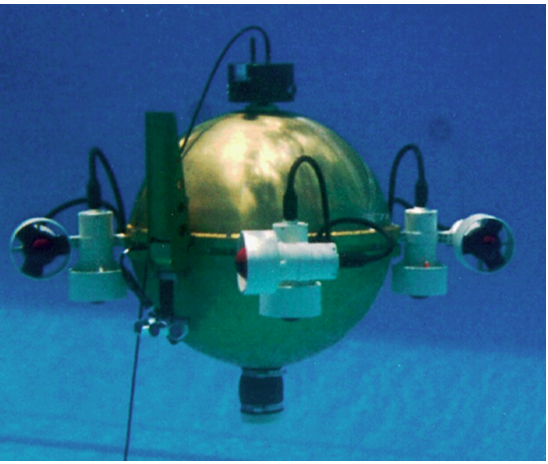
\includegraphics[width=0.25\linewidth]{img/ODIN2.png}};
	\end{tikzpicture}
\end{frame}




% =========================================
% =========================================




\begin{frame}{An example of the ODIN}
	\framesubtitle{Rigid body equation of motion}
	Dynamic equations
	\begin{align}
		M_{RB}\dot{\nu} + C_{RB}\nu = \tau_{RB}
	\end{align}
	where
	\begin{align}
		M_{RB} = \begin{bmatrix}
			mI_{3\times 3} & -mS(r_g^b) \\
			mS(r_g^b) & I_b
		\end{bmatrix}; C_{RB} = \begin{bmatrix}
			mS(\nu_2) & -mS(\nu_2)S(r_g^b) \\
			mS(\nu_2)S(r_g^b) & -S(I_b\nu_2)
		\end{bmatrix} \notag
	\end{align}
	Notice that, the term $C_{RB}(\nu)$ is modified by several mathematical transformations such as $C_{RB}(\nu) = C_{RB}(\nu_r)$ by linear velocity -independent parametrizations. Thus, the above dymanic equation could be represented as 
	\begin{align}
		M_{RB}\dot{\nu}_r + C_{RB}\nu_r = \tau_{RB}
	\end{align}
	with $\nu_r$ is the relative velocity of the vehicle. Therefore, the kinematics equation is represented as
	\begin{align}
		\dot{\eta} = J(\eta)\nu
	\end{align}
	where $J(\eta)$ is the Jacobian matrix.
\end{frame}



% =========================================
% =========================================




\begin{frame}{An example of the ODIN}
	\framesubtitle{Added mass}
	In order to lose the general, let's consider the ODIN as a spherical solid. Thus, the ODIN-geometry could be described as the following equation
	\begin{align}
		\dfrac{x^2}{a^2} + \dfrac{y^2}{b^2} + \dfrac{z^2}{c^2} = 0
	\end{align}
	Let's define \footnote{Lamb, Horace. Hydrodynamics. University Press, 1924.}
	\begin{align}
		\alpha_0 = abc \int_0^\infty \frac{\mathrm{d}\lambda}{(a^2 + \lambda) \, \Delta}, \quad
		\beta_0 = abc \int_0^\infty \frac{\mathrm{d}\lambda}{(b^2 + \lambda) \, \Delta}, \quad
		\gamma_0 = abc \int_0^\infty \frac{\mathrm{d}\lambda}{(c^2 + \lambda) \, \Delta}
	\end{align}
	with $\Delta = \big\{(a^2 + \lambda)(b^2 + \lambda)(c^2 + \lambda)\big\}^{\frac{1}{2}}$
	
	\textbf{Special case:} $a = b = c = R$, it is easy to achieve that 
	\begin{align}
		\alpha_0 = \beta_0 = \gamma_0 = R^3 \int\limits_0^\infty \frac{\mathrm{d}\lambda}{(R^2 + \lambda)^2\sqrt{(R^2 + \lambda)}} = R^3\dfrac{2}{3R^3} = \dfrac{2}{3}
	\end{align}
\end{frame}




% =========================================
% =========================================




\begin{frame}{An example of the ODIN}
	\framesubtitle{Added mass}
	Following \footnote{Imlay, Frederick H. The complete expressions for added mass of a rigid body moving in an ideal fluid. No. Report 1528. 1961.}, the added mass of the spherical-solid underwater vehicle could be represented as
	\begin{align}
		&X_{\dot{u}} = -\frac{\alpha_0}{2 - \alpha_0} \frac{4}{3} \pi \rho abc,\\
		&Y_{\dot{v}} = -\frac{\beta_0}{2 - \beta_0} \frac{4}{3} \pi \rho abc,\\
		&Z_{\dot{w}} = -\frac{\gamma_0}{2 - \gamma_0} \frac{4}{3} \pi \rho abc,\\
		&K_{\dot{p}} = -\frac{1}{5} \frac{(b^2 - c^2)(\gamma_0 - \beta_0)}{2(b^2 - c^2) + (b^2 + c^2)(\beta_0 - \gamma_0)} \frac{4}{3} \pi \rho abc,\\
		&M_{\dot{q}} = -\frac{1}{5} \frac{(c^2 - a^2)(\alpha_0 - \gamma_0)}{2(c^2 - a^2) + (c^2 + a^2)(\gamma_0 - \alpha_0)} \frac{4}{3} \pi \rho abc,\\
		&N_{\dot{r}} = -\frac{1}{5} \frac{(a^2 - b^2)(\beta_0 - \alpha_0)}{2(a^2 - b^2) + (a^2 + b^2)(\alpha_0 - \beta_0)} \frac{4}{3} \pi \rho abc.
	\end{align}
\end{frame}




% =========================================
% =========================================




\begin{frame}{An example of the ODIN}
	\framesubtitle{Added mass}
	\textbf{Special case:} $a = b = c = R$, then $\alpha_0 = \beta_0 = \gamma_0 = \dfrac{2}{3}$, therefore
	\begin{align}
		X_{\dot{u}} = Y_{\dot{v}} = Z_{\dot{w}} = -\rho\dfrac{2}{3}\pi R^3\\
		K_{\dot{p}} = K_{\dot{p}} = K_{\dot{p}} = 0
	\end{align}
	Written in matrix form,
	\begin{align}
		M_A = \begin{bmatrix}
			\rho\dfrac{2}{3}\pi R^3 I_3 & 0_3 \\ 0_3 & 0_3
		\end{bmatrix}
	\end{align}
	Then, it is easy to find the Coriolis term of added mass, which is not depended on $\nu_1$
	\begin{align}
		C_A(\nu_r) = \rho \frac{2}{3} \pi R^3
		\begin{bmatrix}
			0 & 0 & 0 & 0 & w_r & -v_r \\
			0 & 0 & 0 & -w_r & 0 & u_r \\
			0 & 0 & 0 & v_r & -u_r & 0 \\
			0 & w_r & -v_r & 0 & 0 & 0 \\
			-w_r & 0 & u_r & 0 & 0 & 0 \\
			v_r & -u_r & 0 & 0 & 0 & 0
		\end{bmatrix}
	\end{align}
\end{frame}



% =========================================
% =========================================




\begin{frame}{An example of the ODIN}
	\framesubtitle{Gravitational/buoyancy forces}
	Hydrostatics force of Submerged Vehicles is represented as
	\begin{align}
		g(\eta) =
		\begin{bmatrix}
			(W - B) \sin(\theta) \\
			- (W - B) \cos(\theta) \sin(\phi) \\
			- (W - B) \cos(\theta) \cos(\phi) \\
			- (y_g W - y_b B) \cos(\theta) \cos(\phi) + (z_g W - z_b B) \cos(\theta) \sin(\phi) \\
			(z_g W - z_b B) \sin(\theta) + (x_g W - x_b B) \cos(\theta) \cos(\phi) \\
			- (x_g W - x_b B) \cos(\theta) \sin(\phi) - (y_g W - y_b B) \sin(\theta)
		\end{bmatrix}
	\end{align}
	with $(x_g, y_g, z_g)$ and $(x_b, y_b, z_b)$ are the coordinates of CO and CB, respectively.
	
	\textbf{Special case:} 
	\begin{itemize}
		\item $W = B \to$ neutral buoyant, the Gravitational/buoyancy forces just cause the rotations (moments).
		\item $Oz_b$ and $Oz_g$ are coincidence. That mean $x_g = x_b$ and $y_g = y_b$. 
		\item  $CB \equiv CG \equiv CO$ and $W = B \to$ $g(\eta) = (0, 0, 0, 0, 0, 0)^\top$.
	\end{itemize}
\end{frame}



% =========================================
% =========================================




\begin{frame}{An example of the ODIN}
	\framesubtitle{Damping}
	Damping includes
	\begin{itemize}
		\item Linear damping 
		\begin{align}
			D = -diag(X_u, Y_v, Z_w, K_p, M_q, N_r)
		\end{align}
		\item Nonlinear term (important for high-speed vehicles)
		\begin{align}
			d(\nu_r) = \begin{bmatrix}
				\dfrac{1}{2}V_r^2S C_D(\alpha)\cos\alpha - \dfrac{1}{2}V_r^2S C_L(\alpha)\sin\alpha \\
				Y_{cross}\\
				-\dfrac{1}{2}V_r^2S C_D(\alpha)\sin\alpha - \dfrac{1}{2}V_r^2S C_L(\alpha)\cos\alpha \\
				0_{3\times 1}
			\end{bmatrix}
		\end{align}
		More details, $C_D$, $C_L$ are the drag, lifting coefficient, respectively.
		\begin{align}
			&F_{drag} = -\dfrac{1}{2}\rho V_r^2 S C_D(\alpha)\\
			&F_{lift} = -\dfrac{1}{2}\rho V_r^2 S C_L(\alpha)\\
			&Y_{cross} = -\dfrac{1}{2}\rho
			\int\limits_{-L/2}^{L/2}T(x)C_d^{2D}(x)|v_r + xr|(v_r + xr)dx
		\end{align}
		
		The sideslip angle ($\beta$) and attack angle ($\alpha$) is defined in slide \ref{slide: Transformation between BODY and FLOW}.
	\end{itemize}
\end{frame}


% =========================================
% =========================================




\section{Guidance - Navigation - Control}

\begin{frame}{Guidance - Navigation - Control}
	\framesubtitle{GNC overview}
	In the previous section, we introduce the modeling and mathematical model to describe the dynamics behavior. In the following steps, the control techniques, which include guidance, navigation and motion control, for a specific underwater vehicle (in general, consider the ocean vehicle).  The theory and cases studies are organized as three independent part:
	\begin{itemize}
		\item \textbf{G -  Guidance Systems}: Systems for automatically guiding the path of a marine craft, usually without direct or continuous human control.
		\item \textbf{N -  Navigation Systems}: Systems for determination of the craft’s position/attitude, velocity and acceleration.
		\item \textbf{C - Control Systems}: PID design methods for automatic control of position/attitude,
		velocity and acceleration. This involves control systems for stabilization, trajectory-tracking and path following control of marine craft.
	\end{itemize}
\end{frame}




% =========================================
% =========================================




\begin{frame}{Guidance - Navigation - Control}
	\framesubtitle{GNC overview}
	\begin{tikzpicture}[remember picture,overlay]
		% \node[fill=blue!30, text=white, font=\large, rounded corners] 
		\node at (current page.north east) [xshift=-6cm, yshift=-3cm] 
		{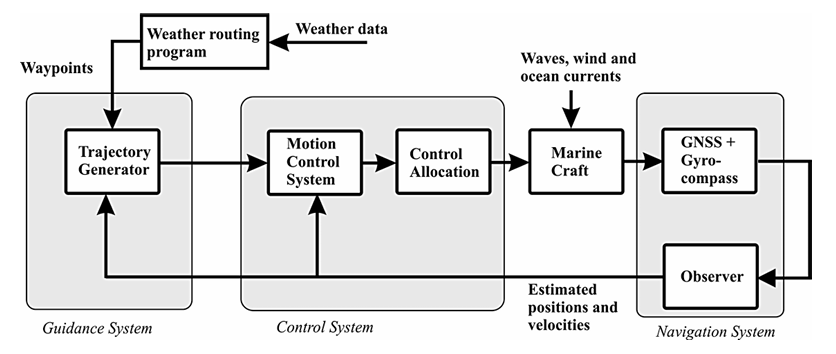
\includegraphics[width=0.7\linewidth]{img/GNC.png}};
	\end{tikzpicture}
	
	\begin{tikzpicture}[remember picture,overlay]
		% \node[fill=blue!30, text=white, font=\large, rounded corners] 
		\node at (current page.north east) [xshift=-6cm, yshift=-7cm] 
		{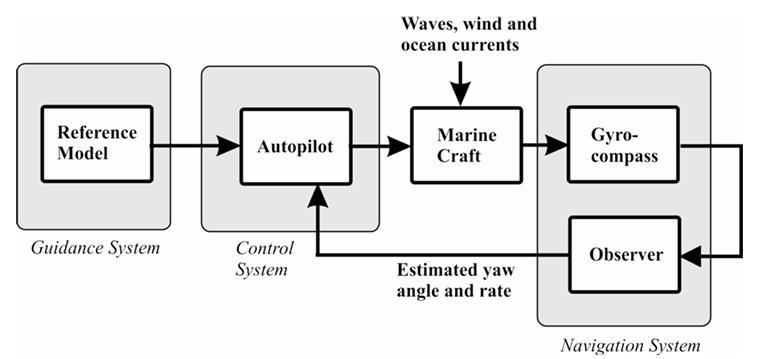
\includegraphics[width=0.7\linewidth]{img/GNC1.png}};
	\end{tikzpicture}
	
\end{frame}






% =========================================
% =========================================




\begin{frame}{Guidance - Navigation - Control}
	\framesubtitle{Setpoint regulation, trajectory-tracking control and path-following control}
	\textbf{Setpoint Regulation:} The most basic guidance system is {\color{red}a constant input or setpoint provided by a human operator}. The corresponding controller will then be a regulator. Examples of setpoint regulation are constant depth, trim, heel and speed control. It could also be regulation to zero, which is commonly required in roll and pitch for instance.
	
	\textbf{Trajectory-Tracking Control:} The position and velocity of the marine craft should {\color{red}track desired time varying position and velocity reference signals}. The corresponding feedback controller is a trajectory tracking controller. Tracking control can be used for course-changing maneuvers, speed-changing and attitude control. An advanced guidance system computes optimal time-varying trajectories from a dynamic model for a predefined control objective. If a constant setpoint is used as input to a low-pass filter (reference model) in an open-loop guidance system, the outputs of the filter will be smooth time-varying reference trajectories for position, velocity and acceleration (PVA).
	
	\textbf{Path-Following Control:} This is to {\color{red} follow a predefined path independent of time} (no temporal constraints). Moreover, no restrictions are placed on the temporal propagation along the path. This is typical for ships in transit between continents or underwater vehicles used to map the seabed.
\end{frame}



% =========================================
% =========================================




\begin{frame}{Guidance - Navigation - Control}
	\framesubtitle{Guidance - Target tracking}
	\begin{tikzpicture}[remember picture,overlay]
		% \node[fill=blue!30, text=white, font=\large, rounded corners] 
		\node at (current page.north east) [xshift=-6cm, yshift=-3.5cm] 
		{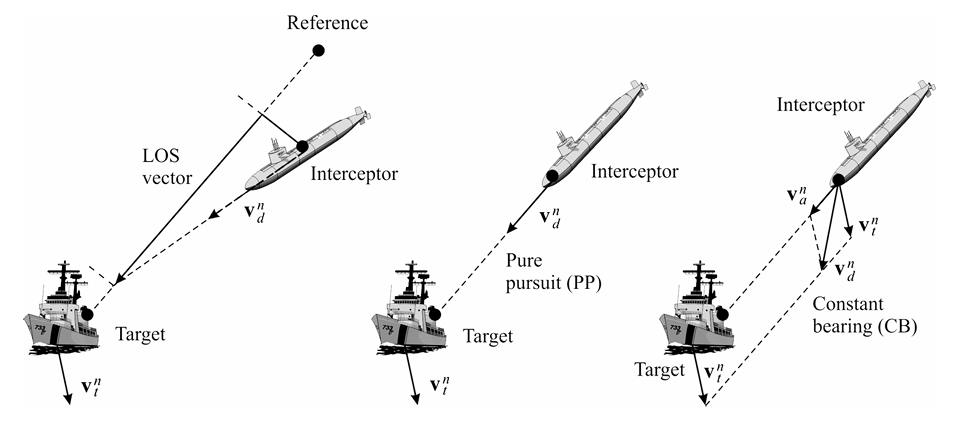
\includegraphics[width=0.8\linewidth]{img/Guidance.png}};
	\end{tikzpicture}
	
	\vspace{3cm}
	Several guidance strategies
	\begin{itemize}
		\item Line-of-Sight Guidance (LOS)
		\item Pure Pursuit Guidance (PP)
		\item Constant Bearing Guidance (CB)
		\item ...
	\end{itemize}
\end{frame}


% =========================================
% =========================================

\begin{frame}{Guidance - Navigation - Control}
	\framesubtitle{Guidance - Trajectory tracking}
	\begin{tikzpicture}[remember picture,overlay]
		% \node[fill=blue!30, text=white, font=\large, rounded corners] 
		\node at (current page.north east) [xshift=-6cm, yshift=-3.5cm] 
		{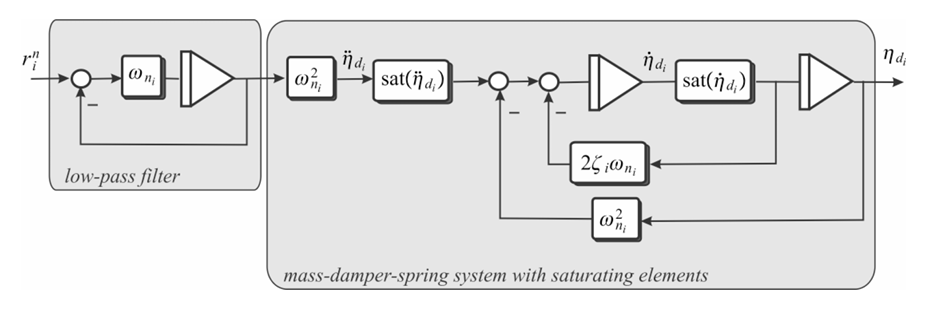
\includegraphics[width=0.8\linewidth]{img/Guidance1.png}};
	\end{tikzpicture}
	
	\vspace{3cm}
	
	The easiest approach is that the desired trajectory can be computed using reference models generated by 	low-pass filters
	\begin{align}
		\dfrac{x_d}{r}(s) = h_{lp}(s) = \dfrac{\omega^2}{s^2 + 2\xi\omega s + \omega^2}
	\end{align}
	where $r(s)$ is set up by operator and $x_d(s)$ is the controller input.
\end{frame}


% =========================================
% =========================================

\begin{frame}{Guidance - Navigation - Control}
	\framesubtitle{Guidance - Trajectory tracking}
	The second one is that we consider the simulation model to generate the trajectory. For instance, a dynamic model could be chosen as
	\begin{align}
		\dot{\eta}_d = J(\eta)\nu_d \\
		M\dot{\nu}_d + N\nu_d + g(\nu_d) = \tau
	\end{align}
	The smooth trajectory could be generated by simulating the above dynamic model with a certain controller, such as PD control. To explain,
	\begin{align}
		\tau = g(\eta_d) - J^{-1}(\eta_d)(K_p(\eta_d - \eta_{ref}) + Kd\dot{\eta}_d)
	\end{align}
\end{frame}



% =========================================
% =========================================

\begin{frame}{Guidance - Navigation - Control}
	\framesubtitle{Guidance - Trajectory tracking}
	The vehicles' trajectory could be generated by optimization problems. The easiest approach method for this problem by consider a cost function of power, or time, and the purpose is to minimize this cost function. That mean,
	\begin{align}
		x_d* = \text{argmin}_{x_d}\Big(f(x, t)\Big) \\
		s.t. \quad x_d \in \mathcal{X} 
	\end{align}
	For examples, by considering the discrete model of vehicles, the optimization problem could be expressed in detail as follows 
	\begin{align}
		x_d^* = \text{argmin}_{x_d}\sum x_d(k)^\top Q x_d(k)\\
		or\\
		x_d^* = \text{argmin}_{x_d} t
	\end{align}
	with constraint $x_d(k+1) = f(x_d(k), u(k))$ and $Q = Q^\top > 0$
\end{frame}


% =========================================
% =========================================

\begin{frame}{Guidance - Navigation - Control}
	\framesubtitle{Guidance - Path following}
	Path generation using straight lines and Circular Arcs
	
	\textit{ The shortest path (minimum time) between two configurations $(x, y, \psi)$ of a craft moving at constant speed U is a path formed by straight lines and circular arc segments.}
	
	\vspace{5cm}
	
	\begin{tikzpicture}[remember picture,overlay]
		% \node[fill=blue!30, text=white, font=\large, rounded corners] 
		\node at (current page.north east) [xshift=-3cm, yshift=-6cm] 
		{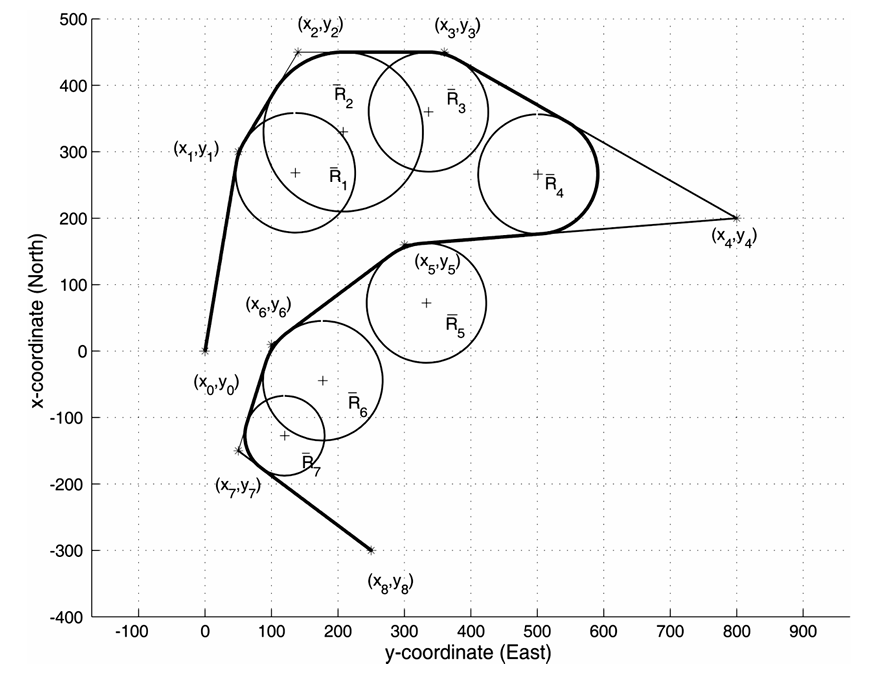
\includegraphics[width=0.5\linewidth]{img/path_gen.png}};
	\end{tikzpicture}
	
	\begin{tikzpicture}[remember picture,overlay]
		% \node[fill=blue!30, text=white, font=\large, rounded corners] 
		\node at (current page.north east) [xshift=-9.5cm, yshift=-6cm] 
		{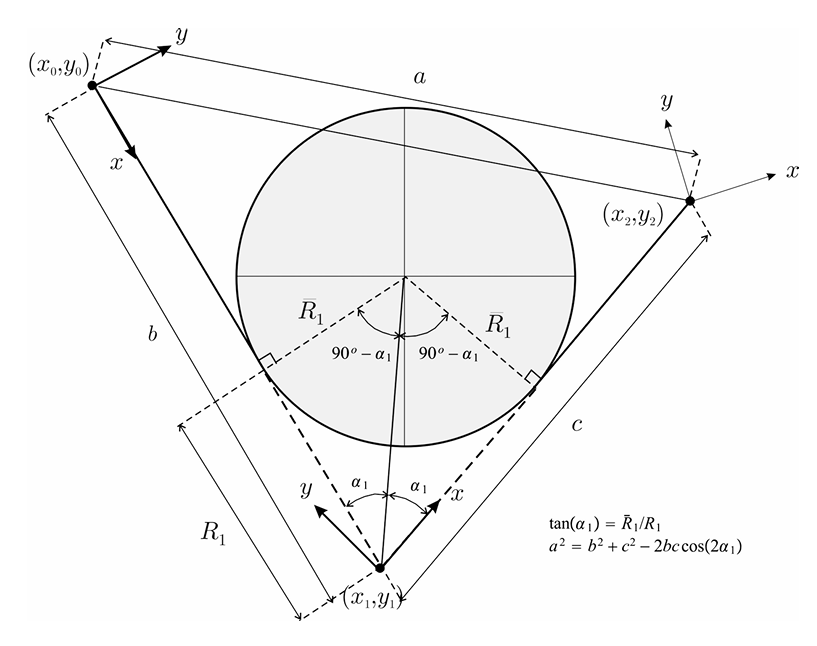
\includegraphics[width=0.5\linewidth]{img/path_gen1.png}};
	\end{tikzpicture}
	
\end{frame}


% =========================================
% =========================================

\begin{frame}{Guidance - Navigation - Control}
	\framesubtitle{Guidance - Path following}
	First of all, we consider \textbf{a Straight-line path} and introduce two different guidance principles, which could be used to steer along the LOS vector:
	\begin{itemize}
		\item Enclosure-based steering $\to$ find $(x_{los}, y_{los})$ base on a a circle with radius $R>0$ enclosuring $(x, y)$
		\item Lookahead-based steering $\to$ steering law could be easy to modify
	\end{itemize}
	
	\vspace{5cm}
	
	
	
	\begin{tikzpicture}[remember picture,overlay]
		% \node[fill=blue!30, text=white, font=\large, rounded corners] 
		\node at (current page.north east) [xshift=-9.5cm, yshift=-6.5cm] 
		{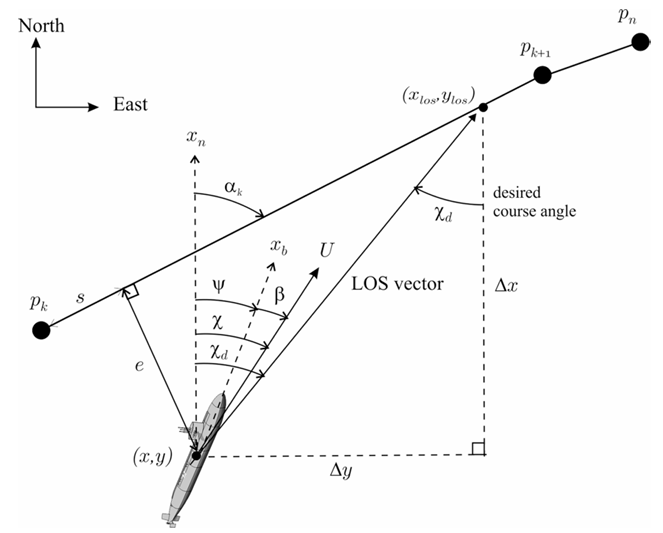
\includegraphics[width=0.5\linewidth]{img/path follow.png}};
	\end{tikzpicture}
	
	
	\begin{tikzpicture}[remember picture,overlay]
		% \node[fill=blue!30, text=white, font=\large, rounded corners] 
		\node at (current page.north east) [xshift=-3.5cm, yshift=-6.5cm] 
		{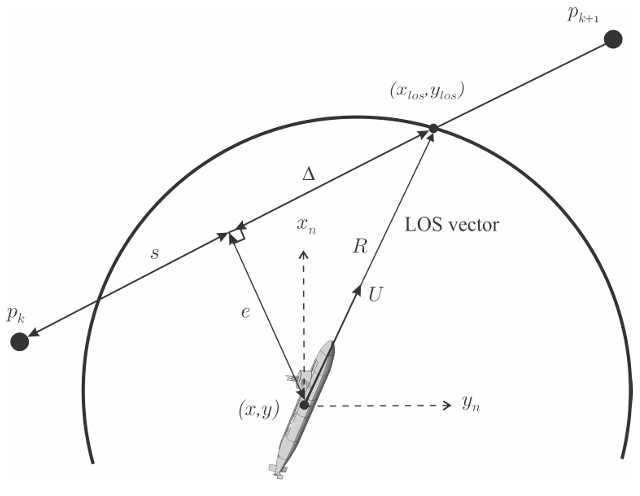
\includegraphics[width=0.5\linewidth]{img/path follow1.png}};
	\end{tikzpicture}
	
\end{frame}



% =========================================
% =========================================

\begin{frame}{Guidance - Navigation - Control}
	\framesubtitle{Guidance - Path following}
	
	
	\begin{tikzpicture}[remember picture,overlay]
		% \node[fill=blue!30, text=white, font=\large, rounded corners] 
		\node at (current page.north east) [xshift=-7cm, yshift=-3.5cm] 
		{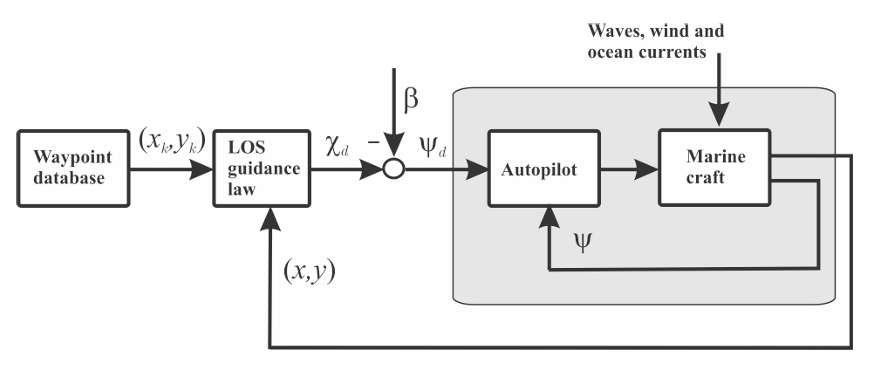
\includegraphics[width=0.8\linewidth]{img/path follow2.png}};
	\end{tikzpicture}
	
	\vspace{3cm}
	
	\begin{itemize}
		\item Enclosure-based steering law $\to$ $\psi_d = atan2(y_{los} - y, x_{los} - x)$
		\item Lookahead-based steering law $\to$ $\psi_d = \chi_d - \beta = \alpha_k + arctan(-\text{PID}(e)) - \beta$
	\end{itemize}
	\textbf{Repeat again:} $\beta$ is the sideslip angle, which calculated by $\beta = arcsin(v/U)$
	
\end{frame}




% =========================================
% =========================================

\begin{frame}{Guidance - Navigation - Control}
	\framesubtitle{Guidance - Path following}
	In the following, \textbf{Path-Following for Curved Paths} is introduced.
	
	MATLAB provide different methods for interpolation. For example, three methods for path generation are the cubic spline interpolant (\texttt{spline.m}), piecewise cubic Hermite interpolanting polynomial (\texttt{pchip.m}) and modified Akima piecewise cubic Hermite interpolation (\texttt{makima.m})
	
	\vspace{4cm}
	
	
	\begin{tikzpicture}[remember picture,overlay]
		% \node[fill=blue!30, text=white, font=\large, rounded corners] 
		\node at (current page.north east) [xshift=-9.5cm, yshift=-6.5cm] 
		{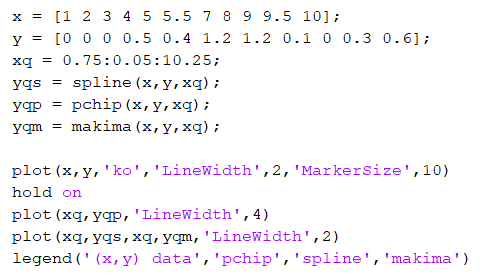
\includegraphics[width=0.5\linewidth]{img/path follow4.png}};
	\end{tikzpicture}
	
	
	\begin{tikzpicture}[remember picture,overlay]
		% \node[fill=blue!30, text=white, font=\large, rounded corners] 
		\node at (current page.north east) [xshift=-3.5cm, yshift=-6.5cm] 
		{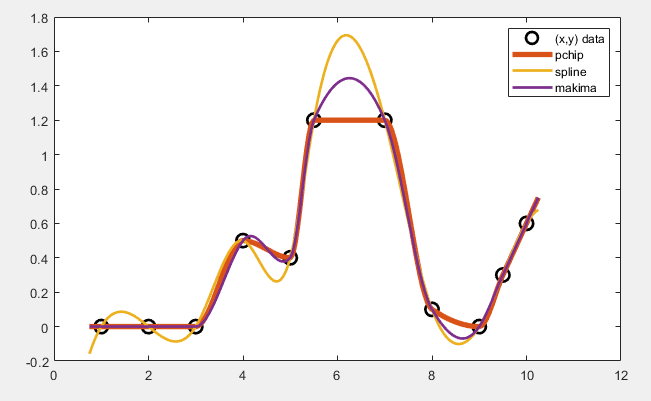
\includegraphics[width=0.5\linewidth]{img/path follow3.png}};
	\end{tikzpicture}
\end{frame}






% =========================================
% =========================================


\begin{frame}{Guidance - Navigation - Control}
	\framesubtitle{Guidance - Path following}
	In other approach, which is called cubic polynomials, we consider a parametrized path as follows
	\begin{align}
		x_d(\varpi) = \sum\limits_{i = 0}^3 a_i\varpi^i; \qquad y_d(\varpi) = \sum\limits_{i = 0}^3 b_i\varpi^i
	\end{align}
	Then, the above constraints must be satisfied
	\begin{align}
		x_d(\varpi_{k-1}) = x_{k - 1}, \quad x_d(\varpi_{k}) = x_{k},\\
		\lim\limits_{\varpi \to \varpi_{k}^{-}} \dfrac{d\,x_d(\varpi_{k})}{d\,\varpi_{k}} = \lim\limits_{\varpi \to \varpi_{k}^{+}} \dfrac{d\,x_d(\varpi_{k})}{d\,\varpi_{k}}\\
		\lim\limits_{\varpi \to \varpi_{k}^{-}} \dfrac{d^2\,x_d(\varpi_{k})}{(d\,\varpi_{k})^2} = \lim\limits_{\varpi \to \varpi_{k}^{+}} \dfrac{d^2\,x_d(\varpi_{k})}{(d\,\varpi_{k})^2}\\
		\dfrac{d\,x_d(\varpi_{k})}{d\,\varpi_{k}}(\varpi_0) = const, \quad \dfrac{d\,x_d(\varpi_{k})}{d\,\varpi_{k}}(\varpi_n) = const\\
		OR \quad \Bigg(\dfrac{d^2\,x_d(\varpi_{k})}{(d\,\varpi_{k})^2}(\varpi_0) = const, \quad \dfrac{d^2\,x_d(\varpi_{k})}{(d\,\varpi_{k})^2}(\varpi_n) = const\Bigg)
	\end{align}
\end{frame}





% =========================================
% =========================================

\begin{frame}{Guidance - Navigation - Control}
	\framesubtitle{Guidance - Path following}
	\begin{tikzpicture}[remember picture,overlay]
		% \node[fill=blue!30, text=white, font=\large, rounded corners] 
		\node at (current page.north east) [xshift=-6.5cm, yshift=-5cm] 
		{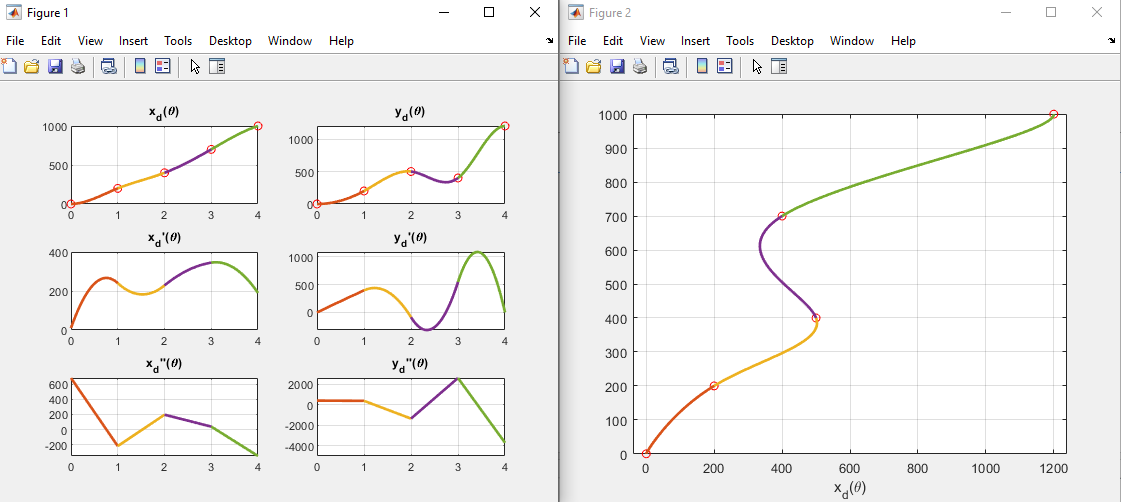
\includegraphics[width=\linewidth]{img/path follow5.png}};
	\end{tikzpicture}
	
\end{frame}




% =========================================
% =========================================

\begin{frame}{Guidance - Navigation - Control}
	\framesubtitle{Guidance - Path following}
	\textbf{Transformation of Path to Reference Trajectories using Desired Speed Profiles}
	
	\begin{align}
		\dot{\varpi}(t) = \dfrac{U_d(t)}{\sqrt{\dfrac{d\,x_d(\varpi_{k})}{d\,\varpi_{k}}(\varpi)^2 + \dfrac{d\,x_d(\varpi_{k})}{d\,\varpi_{k}}(\varpi)^2}}\\
		T\dot{U}_d(t) + U_d(t) = U_{ref}
	\end{align}
	
	
\end{frame}



% =========================================
% =========================================

\begin{frame}{Guidance - Navigation - Control}
	\framesubtitle{Guidance - Path following}
	In another view, the cubic polynomials approach could be formed by the \textbf{Nonlinear Constrained Optimization Problem}. Firstly, the constraint of the cubic polynomials approach could be represented by the the linear form
	\begin{align}
		y = A(t_k, t_{k + 1})x
	\end{align}
	where $x$ is the vector of polynomial coefficients, and $y$, $A$ are the derived constraints vector and matrix. Then, the optimization problem is formed
	\begin{align}
		\text{minimize} \Big[\Big(A(t_k, t_{k + 1})x - y\Big)^\top\Big(A(t_k, t_{k + 1})x - y\Big)\Big]
	\end{align}
	with the constraint of velocities and accelerations.
\end{frame}




% =========================================
% =========================================

\begin{frame}{Guidance - Navigation - Control}
	\framesubtitle{Guidance - Path following}
	
	\begin{columns}[onlytextwidth]
		\column{.5\textwidth}
		The solution to the problem of path-following proposed here builds on the following intuitive explanation a simple path-following controller should compute 
		
		(i) the distance between the vehicle’s center of mass $Q$ and a point $P$, and 
		
		(ii) the angle between the vehicle’s total velocity vector $v_t$ and the tangent to the path at $P$, and reduce both to zero. This motivates the development of the `kinematic' model of the vehicle in terms of a Serret–Frenet frame $\{F\}$ that moves along the path; $\{F\}$ plays the role of the body axis of a ‘virtual target vehicle’ that should be tracked by the `real vehicle'.
		\column{.5\textwidth}
	\end{columns}
	
	
	\begin{tikzpicture}[remember picture,overlay]
		% \node[fill=blue!30, text=white, font=\large, rounded corners] 
		\node at (current page.north east) [xshift=-3cm, yshift=-5cm] 
		{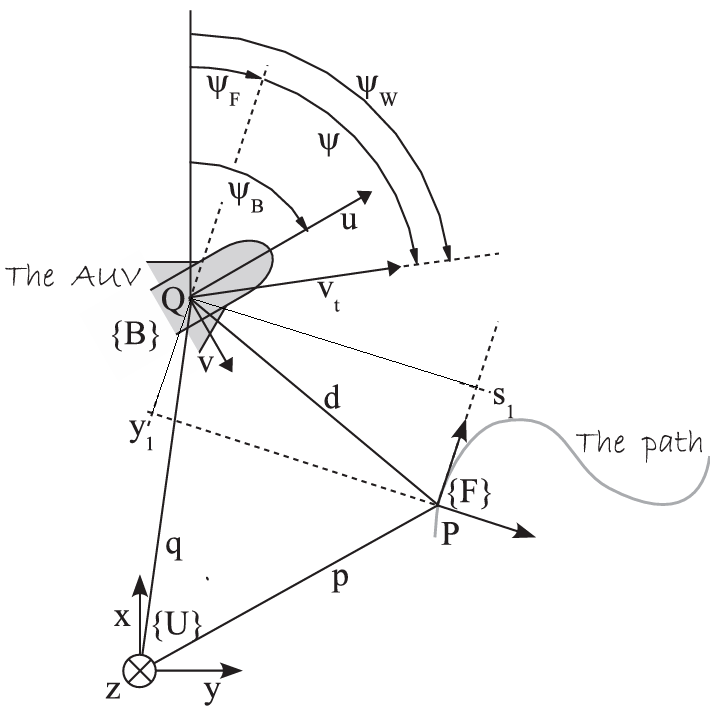
\includegraphics[width=0.5\linewidth]{img/path follow6.png}};
	\end{tikzpicture}
	
\end{frame}




% =========================================
% =========================================

\begin{frame}{Guidance - Navigation - Control}
	\framesubtitle{Guidance - Path following}
	
	\begin{columns}[onlytextwidth]
		\column{.5\textwidth}
		\small
		\begin{align}
			\dot{s}_1 &= -\dot{s}(1 - c_c y_1) + v_t \cos\psi, \\
			\dot{y}_1 &= -c_c \dot{s}_1 + v_t \sin\psi, \\
			\dot{\psi} &= r + \dot{\beta}- c_c \dot{s}.
		\end{align}
		
		Assuming we have a precise estimation of the function $\mu(s)$, and given $s$, we compute
		\begin{align}
			x_s(\mu) = \sum_{i=1}^n a_i \mu^i, \quad y_s(\mu) = \sum_{i=1}^n b_i \mu^i,\\
			\psi_F(s) = \arctan\left(\frac{(y_s)'}{(x_s)'}\right), \\
			c_c(s) = \frac{\partial \psi_F(s)}{\partial \mu} \frac{d\mu}{ds}, \\
			\frac{\partial c_c(s)}{\partial s} = \frac{\partial c_c(s)}{\partial \mu} \frac{d\mu}{ds}, \\
			(x_s)' = \frac{dx_s}{d\mu}, \quad (y_s)' = \frac{dy_s}{d\mu}\\
			\frac{d\mu}{ds} = \frac{1}{\sqrt{[(x_s)']^2 + [(y_s)']^2}}.
		\end{align}
		\column{.5\textwidth}
	\end{columns}
	
	
	\begin{tikzpicture}[remember picture,overlay]
		% \node[fill=blue!30, text=white, font=\large, rounded corners] 
		\node at (current page.north east) [xshift=-3.2cm, yshift=-5cm] 
		{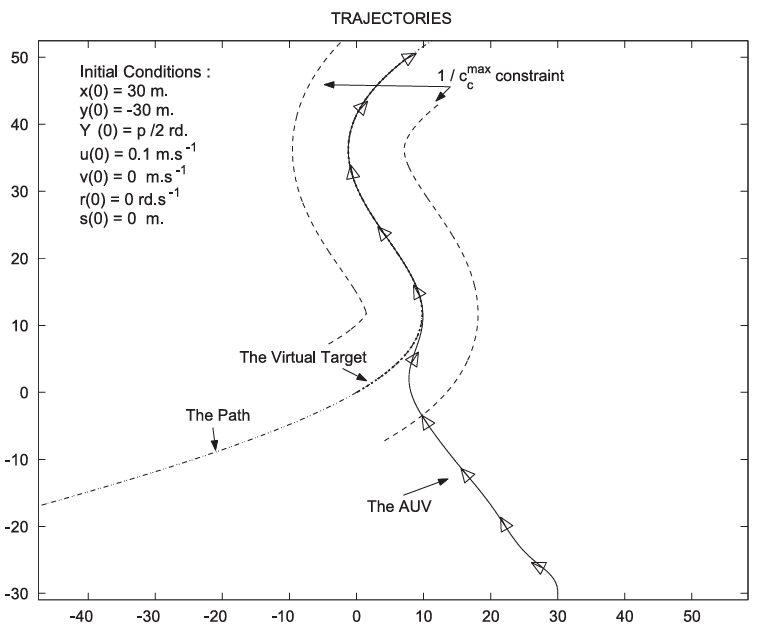
\includegraphics[width=0.5\linewidth]{img/path follow7.png}};
	\end{tikzpicture}
	
\end{frame}






% =========================================
% =========================================

\begin{frame}{Guidance - Navigation - Control}
	\framesubtitle{Navigation}
	\begin{tikzpicture}[remember picture,overlay]
		% \node[fill=blue!30, text=white, font=\large, rounded corners] 
		\node at (current page.north east) [xshift=-6cm, yshift=-3cm] 
		{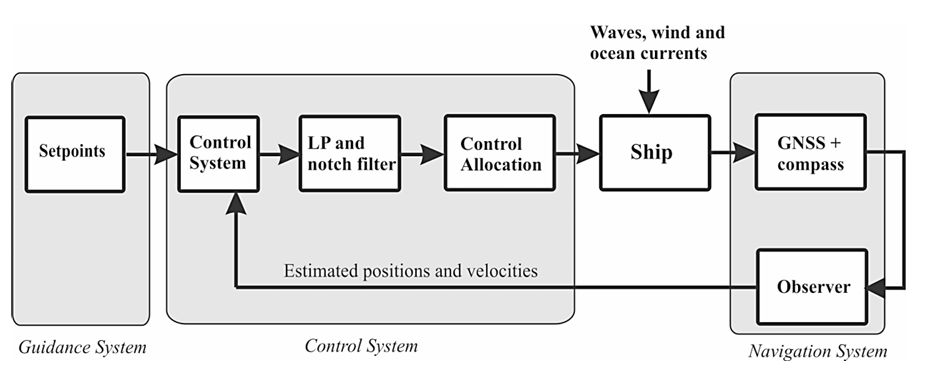
\includegraphics[width=0.7\linewidth]{img/navigation.png}};
	\end{tikzpicture}
	
	\begin{tikzpicture}[remember picture,overlay]
		% \node[fill=blue!30, text=white, font=\large, rounded corners] 
		\node at (current page.north east) [xshift=-6cm, yshift=-6.5cm] 
		{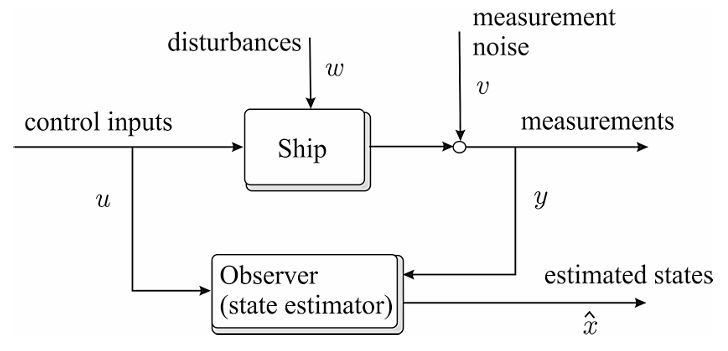
\includegraphics[width=0.6\linewidth]{img/navigation1.png}};
	\end{tikzpicture}
\end{frame}




% =========================================
% =========================================

\begin{frame}{Guidance - Navigation - Control}
	\framesubtitle{Navigation - Low-Pass and Notch filtering}
	\textbf{Low-Pass filtering}: $\omega_b \ll \omega_e$, 
	\begin{align}
		\hat{y}(s) = h_{lp}(s)y(s)
	\end{align}
	where $h_{lp}(s)$ could be chosen as first-order low-pass filter, $h_{lp}(s) = \dfrac{1}{1 + T_fs}$ or the higher-order low-pass filter by using Butterworth filter, $h_{lf}(s) = \dfrac{1}{p(s)}$, with $p(s)p(-s) = 1 + (s/j\omega_f)^{2n}$
	
	\textbf{Cascade Low-Pass and Notch filtering}: 
	\begin{align}
		\hat{y}(s) = h_{lp}(s)h_{n}(s)y(s)
	\end{align}
	with 
	\begin{align}
		h_n(s) = \dfrac{s^2 + 2\xi\omega_ns + \omega_n^2}{(s + \omega_n)^2}; \quad OR \quad h_n(s) = \prod_{i=1}^{3}\dfrac{s^2 + 2\xi\omega_is + \omega_i^2}{(s + \omega_i)^2}
	\end{align}
	
\end{frame}



% =========================================
% =========================================

\begin{frame}{Guidance - Navigation - Control}
	\framesubtitle{Navigation - Observer}
	Consider the linear time-invariant (LTI) system, 
	\begin{align}
		\dot{x} = Ax + Bu\\
		y = Cx
	\end{align}
	and consider its dual system
	\begin{align}
		\dot{\tilde{x}} = A^\top\tilde{x} + C^\top\tilde{u}\\
		\tilde{y} = B^\top\tilde{x}
	\end{align}
	\textbf{Luenberger observer}: coud be designed as \textbf{pole placement control design} for the dual system.

	\textbf{Kalman observer}: coud be designed as \textbf{LQR control design} for the dual system.
	
	Both of above-mentioned observers follow the bellow structure
	\begin{align}
		\dot{z} = Az + Bu + L(y - Cz)
	\end{align}
	with $L$ is observer gain.
	
\end{frame}


% =========================================
% =========================================

\begin{frame}{Guidance - Navigation - Control}
	\framesubtitle{Navigation - Observer}
	In other way, the advance observers that we could approach
	\begin{itemize}
		\item Extended Kalman Filter
		\item High-gain observer
		\item Sliding Mode Observer
		\item Extended State observer
		\item Fixed- and Finite-time observer
		\item ...
	\end{itemize}
	
\end{frame}

% =========================================
% =========================================

\begin{frame}{Guidance - Navigation - Control}
	\framesubtitle{Control - PID control}
	\begin{tikzpicture}[remember picture,overlay]
		% \node[fill=blue!30, text=white, font=\large, rounded corners] 
		\node at (current page.north east) [xshift=-6cm, yshift=-4cm] 
		{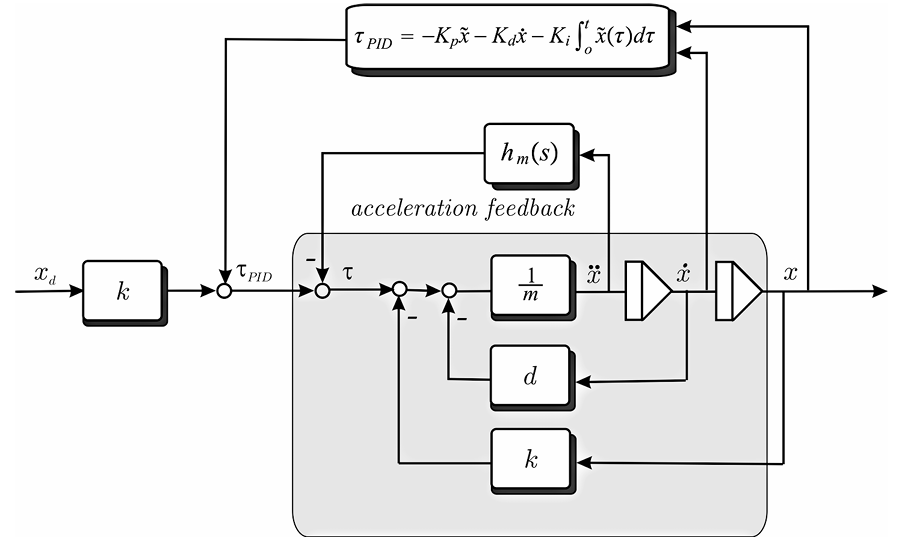
\includegraphics[width=0.7\linewidth]{img/feedback control.png}};
	\end{tikzpicture}
	
	
	\vspace{4.5cm}
	
	Closed-loop feedback system - PID control approach
	\begin{align}
		\tau_{PID} = -K_pe - K_d\dot{e} - K_i\int\limits_{0}^{t}e(\tau)d\tau
	\end{align}
\end{frame}



% =========================================
% =========================================



\begin{frame}{Guidance - Navigation - Control}
	\framesubtitle{Linear control approach}
	In the below section, we approach the control problem of linear system by Linear control technique.
	
	First of all, consider the linearization algorithm for nonlinear system, 
	
	\vspace{1cm}
	
	\begin{minipage}{.5\textwidth}
		\hspace{0cm}
		Assume that, the linear function at $B$ is
		\begin{align}
			y &= a_Bx + b_B \\
			&\approx F(x) \Big|_{x \in \Delta_{x_B}}
		\end{align}
		where $a_B$ is the coefficient of first degree, easy to determine
		\begin{align}
			a_B = \dfrac{\partial F(x)}{\partial x}\Bigg|_{x = x_B}
		\end{align}
		and $b_B$ is the bias.
	\end{minipage}%
	\begin{minipage}{.5\textwidth}
		\hspace{+0.25cm}
		\centering
		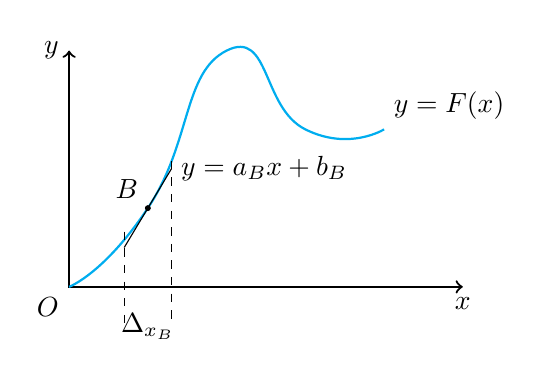
\begin{tikzpicture}
			% \draw (0, 0) grid (5, 5);
			\draw [<->, thick] (5, 0) node[below]{$x$} -- (0, 0) node[below left]{$O$} -- (0, 3) node[left]{$y$};
			\draw [cyan, thick] plot [smooth, tension=1] coordinates { (0,0) (1,1) (2,3) (3,2) (4,2)};
			\draw (4, 2) node[above right] {$y = F(x)$};
			\coordinate (A) at (3, 2);
			\coordinate (B) at (1, 1);
			\draw [fill = black] (B) node[above left] {$B$} circle (0.03);
			
			\draw (0.7, 0.5) -- (1.3, 1.5) node [right] {$y = a_Bx + b_B$};
			\draw [dashed] (0.7, 0.7) -- (0.7, -0.5);
			\draw [dashed] (1.3, 1.6) -- (1.3, -0.5);
			\draw (1, -0.5) node {$\Delta_{x_B}$};
			
		\end{tikzpicture}
	\end{minipage}
\end{frame}

% =========================================
% =========================================


\begin{frame}{Guidance - Navigation - Control}
	\framesubtitle{Linear control approach}
	Consider a general system, which found in the above
	\begin{align}
		\Dot{{x}} = f({x}) + g({x})\tau = F({x}, \tau)
	\end{align}
	$\to$ Let's approximate it to the linear original difference equation (ODE)
	\begin{align}
		\Dot{{x}} = {A}{x} + {B}\tau
	\end{align}
	where, the state-space matrices are defined as
	\begin{align}
		{A} = \dfrac{\partial F({x}, \tau)}{\partial {x}}\Bigg|_{{x} = {x}_e,\tau = \tau_e} \\
		{B} = \dfrac{\partial F({x}, \tau)}{\partial \tau}\Bigg|_{{x} = {x}_e, \tau = \tau_e}
	\end{align}
\end{frame}

% =========================================
% =========================================





\begin{frame}{Guidance - Navigation - Control}
	\framesubtitle{State-Space-based Linear control approach}
	{\color{red} In the following step, we propose a linear control technique - pole placement control.}
	
	\vspace{0.5cm}
	
	First, consider the state-space model, described as follows
	\begin{align}
		\Dot{{x}} = {A}{x} + {B}\tau \label{eqn: system}
	\end{align}
	As mention above, the control signal is 
	\begin{align}
		\tau = h({x})
	\end{align}
	such as, the system in (\ref{eqn: system}) is stable.\\ 
	For simplify the control signal, we assume that, the control law is a gain of state variables
	\begin{align}
		\tau = h({x}) = -{K}{x}
	\end{align}
	{\color{red} This is the most simplify of control law!}
\end{frame}



% =========================================
% =========================================



\begin{frame}{Guidance - Navigation - Control}
	\framesubtitle{State-Space-based Linear control approach}
	With the control signal defined as $\tau = h({x}) = -{K}{x}$, the close-loop system becomes
	\begin{align}
		\Dot{{x}} &= {A}{x} - {B}{K}{x} \\
		& = ({A} - {B}{K}){x}
	\end{align}
	Let $\Tilde{{A}} = {A} - {B}{K}$. This ODE exist the solution as
	\begin{align}
		{x} = \text{e}^{\Tilde{{A}}t} = \sum\limits_{i = 0}^{\infty}\dfrac{\Tilde{{A}}^it^i}{i!} = {P}^{-1}\Big(\sum\limits_{i = 0}^{\infty}\dfrac{{L}^it^i}{i!} \Big) {P}=  {P}^{-1}\text{e}^{{L}t} {P}
	\end{align}
	where 
	\begin{align}
		{L} = diag(\lambda_1, \lambda_2, ..., \lambda_i)
	\end{align}
	$\lambda_i$ are the eigenvalue of $\Tilde{{A}}$ with eigenvector ${P}_i$ and
	\begin{align}
		{P} = \begin{bmatrix}
			{P}_1^\top & {P}_2^\top & ... & {P}_i^\top
		\end{bmatrix}^\top
	\end{align}\\
	{\color{red} Find ${K}$ such as $\lim_{t \to \infty}{x} = 0$ that mean Find ${K}$ such as ${L} < 0$}
\end{frame}






% =========================================
% =========================================



\begin{frame}{Guidance - Navigation - Control}
	\framesubtitle{State-Space-based Linear control approach}
	{\color{red} Similarly, by considering a optimization problem, Linear Quadratic Regulator is constructed.}
	
	
	First of all, consider linear time-invariant system
	\begin{align}
		\dfrac{d}{dt}{x} = {A}{x} + {B}u
	\end{align}
	and control signal for this system
	\begin{align}
		{u} = {\omega} - G{x}
	\end{align}
	The LQR controller is a state feedback controller, with the control signal $u$ found to be satisfied
	\begin{align}
		J = \dfrac{1}{2}\int\limits_{0}^\infty\Big({x}^T{Q}{x} + {u}^T{Ru}\Big)\text{d}t \to \min \label{eqn:cost_function}
	\end{align}
	$J$ is the cost function, ${Q} = {Q}^T > 0$ and ${R} = {R}^T > 0$ are weight matrices.
\end{frame}




% =========================================
% =========================================



\begin{frame}{Guidance - Navigation - Control}
	\framesubtitle{State-Space-based Linear control approach}
	\begin{tikzpicture}[remember picture,overlay]
		% \node[fill=blue!30, text=white, font=\large, rounded corners] 
		\node at (current page.north east) [xshift=-6cm, yshift=-3.5cm] 
		{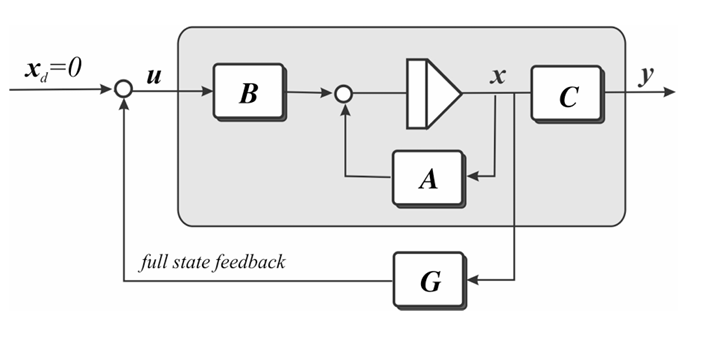
\includegraphics[width=0.7\linewidth]{img/feedback control1.png}};
	\end{tikzpicture}
	
	\vspace{3.5cm}
	
	
	The first step to find the LQR controller is to find the solution ${P} = {P}^T > 0$ of the Algebraic Riccati Equation (ARE)
	\begin{align}
		{P}{A} + {A}^T{P} - {P}{B}{R}^{-1}{B}^T{P} + {Q} = 0
	\end{align}
	then, the controller matrix $G$ can be found 
	\begin{align}
		G = {R}^{-1}{B}^T{P}
	\end{align}
	
	
	
	
\end{frame}



% =========================================
% =========================================


\begin{frame}{Guidance - Navigation - Control}
	\framesubtitle{Nonlinear control approach}
	{\color{red} In the following section, a basic nonlinear control strategy that based on Sliding Mode Control is introduced.}
	
	
	For nonlinear control strategy, we consider the Sliding Mode Control technique. First of all, the control purpose is that the state variables track the desired states. That means if we consider the system, which is described by the above ODE
	\begin{align}
		\ddot{{x}} = f({x}, \dot{{x}}) + g({x}, \dot{{x}})\tau
	\end{align}
	Assume that, the desired states is defined by ${x}_d$. Then, the error states are
	\begin{align}
		{e} = {x} - {x}_d; \quad \dot{{e}} = \dot{{x}} - \dot{{x}}_d
	\end{align}
	Then, we define a sliding variable and a sliding surface with positive definite matrix ${k} > 0$ as follows
	\begin{align}
		{s} = \dot{{e}} + {k}{e} ; \quad \mathcal{S} = \{{x}, \dot{{x}} | {s} = {0}\}
	\end{align}
	{\color{red} Notice that, by choosing a positive definite matrix ${k}$, this is easy to achieve that ${s} \to {0}$ then ${e} \to {0}$ and $\dot{{e}} \to {0}$}
\end{frame}




% =========================================
% =========================================


\begin{frame}{Guidance - Navigation - Control}
	\framesubtitle{Nonlinear control approach}
	In the following step, a control law is proposed to act the sliding variables to the sliding surface. First, we consider the Lyapunov candidate as follows
	\begin{align}
		V = \dfrac{1}{2}{s}^\top{s} \quad > 0
	\end{align}
	And its derivative could be easy to achieve
	\begin{align}
		\dot{V} = {s}^\top\dot{{s}} = {s}^\top(\ddot{{x}} - \ddot{{x}}_d + {k}\dot{{e}}) \notag\\
		= {s}^\top(f({x}, \dot{{x}}) + g({x}, \dot{{x}})\tau - \ddot{{x}}_d + {k}\dot{{e}})
	\end{align}
	Following Lyapunov stability theorem, let's choose the control signal as 
	\begin{align}
		\tau = g({x}, \dot{{x}})^{-1}\big(-f({x}, \dot{{x}}) + \ddot{{x}}_d - {k}\dot{{e}} - \eta{s} - \gamma sign({s})\big)
	\end{align}
	then, the derivative of Lyapunov candidate becomes
	\begin{align}
		\dot{V} = {s}^\top(-\eta{s} - \gamma sign({s})) = -{s}^\top\eta{s} - \gamma |{s}|
	\end{align}
	$\to$ if $\eta$ and $\gamma$ are positive definite, $\dot{V} < 0$, thus, ${s} \to {0}$
\end{frame}



% =========================================
% =========================================


\begin{frame}{Guidance - Navigation - Control}
	\framesubtitle{Nonlinear control approach}
	\begin{tikzpicture}[remember picture,overlay]
		% \node[fill=blue!30, text=white, font=\large, rounded corners] 
		\node at (current page.north east) [xshift=-9cm, yshift=-4cm] 
		{\includegraphics[width=0.5\linewidth]{img/SMC.png}};
	\end{tikzpicture}
	
	\begin{tikzpicture}[remember picture,overlay]
		% \node[fill=blue!30, text=white, font=\large, rounded corners] 
		\node at (current page.north east) [xshift=-3cm, yshift=-4cm] 
		{\includegraphics[width=0.5\linewidth]{img/SMC1.png}};
	\end{tikzpicture}
	
	\vspace{4cm}
	
	\begin{itemize}
		\item Phase 1: The sliding variables reach the sliding surface, where the sliding variables are zeros
		\item Phase 2: The state errors reach to zeros such that $\dot{{e}} + {k}{e} = 0$
	\end{itemize}
	

\end{frame}


% =========================================
% =========================================


\begin{frame}{Guidance - Navigation - Control}
	\framesubtitle{Forces and Moments allocation}
	Need a map from actuator to Force and Moment. That means
	\begin{align}
		\text{Forces and Moments at center of mass: } \tau \in \mathbb{R}^6\\
		\text{Actuators: } u \in \mathbb{R}^n\\
		\text{Forces and Moments allocation: } f: \mathbb{R}^n \mapsto \mathbb{R}^6
	\end{align}
	
	\vspace{5cm}
	
	\begin{tikzpicture}[remember picture,overlay]
		% \node[fill=blue!30, text=white, font=\large, rounded corners] 
		\node at (current page.north east) [xshift=-7cm, yshift=-7cm] 
		{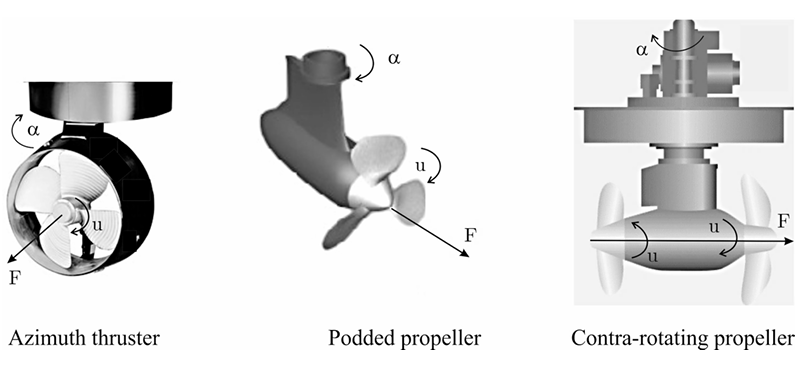
\includegraphics[width=0.8\linewidth]{img/allocation.png}};
	\end{tikzpicture}
\end{frame}



% =========================================
% =========================================


\begin{frame}{Guidance - Navigation - Control}
	\framesubtitle{Forces and Moments allocation}
	\begin{align}
		\text{Forces and Moment constraint: } F_{\vec{k}} = \sum\limits_{i} F_i\vec{k}\\
		M_{\vec{k}} = \sum\limits_{i} M_i\vec{k}\\
		M \text{ [Nm]} = F \text{ [N] } \times l \text{ [m]}
	\end{align}
	
	\vspace{6cm}
	
	\begin{tikzpicture}[remember picture,overlay]
		% \node[fill=blue!30, text=white, font=\large, rounded corners] 
		\node at (current page.north east) [xshift=-6cm, yshift=-7cm] 
		{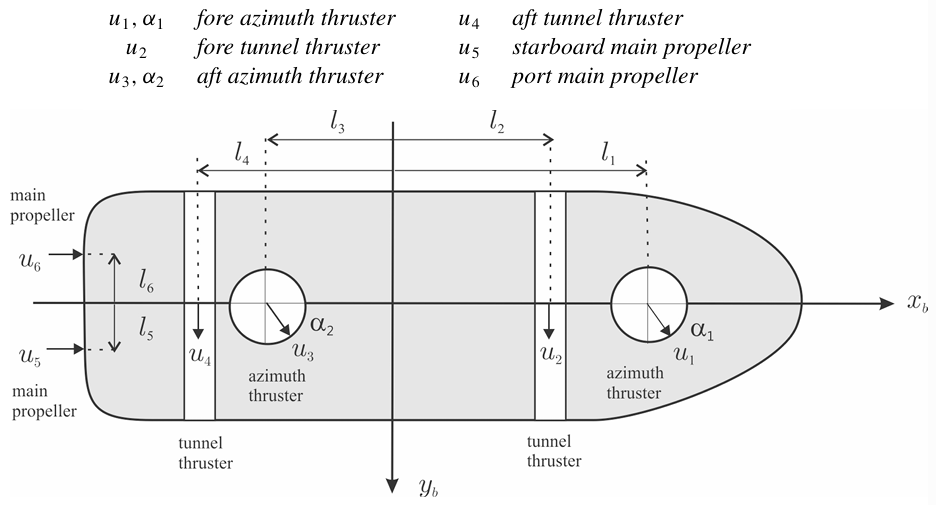
\includegraphics[width=0.8\linewidth]{img/allocation1.png}};
	\end{tikzpicture}
\end{frame}



% =========================================
% =========================================


\section{Numerical simulations}


\begin{frame}{Numerical simulations}
	\framesubtitle{MSS Toolbox}
	The Marine Systems Simulator (MSS) is a Matlab and Simulink library for marine control systems design. The m-files are compatible with the free software GNU Octave. MSS includes models for ships, underwater vehicles, uncrewed surface vehicles, and floating structures. The library also contains guidance, navigation, and control (GNC) blocks for time-domain simulation. 
	
	\vspace{6cm}
	
	\begin{tikzpicture}[remember picture,overlay]
		% \node[fill=blue!30, text=white, font=\large, rounded corners] 
		\node at (current page.north west) [xshift=4cm, yshift=-6cm] {\includegraphics[width=0.5\linewidth]{img/addpath.png}};
	\end{tikzpicture}
	
	
	\begin{tikzpicture}[remember picture,overlay]
		% \node[fill=blue!30, text=white, font=\large, rounded corners] 
		\node at (current page.north west) [xshift=9.5cm, yshift=-6.3cm] {\includegraphics[width=0.5\linewidth]{img/mss_github.png}};
	\end{tikzpicture}
\end{frame}



% =========================================
% =========================================


\begin{frame}{Numerical simulations}
	\framesubtitle{MSS Toolbox}
	The Marine Systems Simulator (MSS) is a Matlab and Simulink library for marine control systems design. The m-files are compatible with the free software GNU Octave. MSS includes models for ships, underwater vehicles, uncrewed surface vehicles, and floating structures. The library also contains guidance, navigation, and control (GNC) blocks for time-domain simulation. 
	
	\vspace{6cm}
	
	\begin{tikzpicture}[remember picture,overlay]
		% \node[fill=blue!30, text=white, font=\large, rounded corners] 
		\node at (current page.north west) [xshift=3cm, yshift=-6cm] {\includegraphics[width=0.5\linewidth]{img/contents_MSS.png}};
	\end{tikzpicture}
	
	
	\begin{tikzpicture}[remember picture,overlay]
		% \node[fill=blue!30, text=white, font=\large, rounded corners] 
		\node at (current page.north west) [xshift=9.5cm, yshift=-6.3cm] {\includegraphics[width=0.5\linewidth]{img/contents_MSS1.png}};
	\end{tikzpicture}
\end{frame}

% =========================================
% =========================================


\begin{frame}{Numerical simulations}
	\framesubtitle{MSS Toolbox}
	Simulink models are constructed by MATLAB R2024
	
	\vspace{6cm}
	
	\begin{tikzpicture}[remember picture,overlay]
		% \node[fill=blue!30, text=white, font=\large, rounded corners] 
		\node at (current page.north west) [xshift=3cm, yshift=-5.5cm] {\includegraphics[width=0.5\linewidth]{img/contents_MSS2.png}};
	\end{tikzpicture}
	
	
	\begin{tikzpicture}[remember picture,overlay]
		% \node[fill=blue!30, text=white, font=\large, rounded corners] 
		\node at (current page.north west) [xshift=9.5cm, yshift=-4.3cm] {\includegraphics[width=0.5\linewidth]{img/contents_MSS3.png}};
	\end{tikzpicture}
	
	\begin{tikzpicture}[remember picture,overlay]
		% \node[fill=blue!30, text=white, font=\large, rounded corners] 
		\node at (current page.north west) [xshift=9.5cm, yshift=-7.3cm] {\includegraphics[width=0.5\linewidth]{img/contents_MSS4.png}};
	\end{tikzpicture}
\end{frame}




% =========================================
% =========================================


\begin{frame}{Numerical simulations}
	\framesubtitle{Example for ODIN}
	Forces distribution
	\vspace{3cm}
	%	\begin{tikzpicture}[remember picture,overlay]
		%		% \node[fill=blue!30, text=white, font=\large, rounded corners] 
		%		\node at (current page.north east) [xshift=-3cm, yshift=-5.5cm] 
		%		{\includegraphics[width=0.4\linewidth]{img/ODIN.png}};
		%	\end{tikzpicture}
	
	\begin{tikzpicture}[remember picture,overlay]
		% \node[fill=blue!30, text=white, font=\large, rounded corners] 
		\node at (current page.north east) [xshift=-3cm, yshift=-5.5cm] 
		{\includegraphics[width=0.4\linewidth]{img/ODIN1.png}};
	\end{tikzpicture}
	
	\begin{tikzpicture}[remember picture,overlay]
		% \node[fill=blue!30, text=white, font=\large, rounded corners] 
		\node at (current page.north east) [xshift=-9cm, yshift=-5.5cm] 
		{\includegraphics[width=0.5\linewidth]{img/force_distri.png}};
	\end{tikzpicture}
\end{frame}





% =========================================
% =========================================


\begin{frame}{Numerical simulations}
	\framesubtitle{Example for ODIN}
	%	\begin{tikzpicture}[remember picture,overlay]
		%		% \node[fill=blue!30, text=white, font=\large, rounded corners] 
		%		\node at (current page.north east) [xshift=-3cm, yshift=-5.5cm] 
		%		{\includegraphics[width=0.4\linewidth]{img/ODIN.png}};
		%	\end{tikzpicture}
	Simulink simulation diagram
	\vspace{7cm}
	
	
	\begin{tikzpicture}[remember picture,overlay]
		% \node[fill=blue!30, text=white, font=\large, rounded corners] 
		\node at (current page.north east) [xshift=-6cm, yshift=-5.5cm] 
		{\includegraphics[width=0.8\linewidth]{img/ODIN_simulink.png}};
	\end{tikzpicture}
\end{frame}



% =========================================
% =========================================


\begin{frame}{Numerical simulations}
	\framesubtitle{Example for ODIN}
	Dynamics and kinematics m-file of ODIN
	\vspace{6cm}
	
	
	\begin{tikzpicture}[remember picture,overlay]
		% \node[fill=blue!30, text=white, font=\large, rounded corners] 
		\node at (current page.north east) [xshift=-9.5cm, yshift=-5.5cm] 
		{\includegraphics[width=0.5\linewidth]{img/ODIN_simulink1.png}};
	\end{tikzpicture}
	
	\begin{tikzpicture}[remember picture,overlay]
		% \node[fill=blue!30, text=white, font=\large, rounded corners] 
		\node at (current page.north east) [xshift=-3cm, yshift=-5.5cm] 
		{\includegraphics[width=0.4\linewidth]{img/ODIN_simulink2.png}};
	\end{tikzpicture}
	
\end{frame}




% =========================================
% =========================================


\begin{frame}{Numerical simulations}
	\framesubtitle{Example for ODIN}
	%	\begin{tikzpicture}[remember picture,overlay]
		%		% \node[fill=blue!30, text=white, font=\large, rounded corners] 
		%		\node at (current page.north east) [xshift=-3cm, yshift=-5.5cm] 
		%		{\includegraphics[width=0.4\linewidth]{img/ODIN.png}};
		%	\end{tikzpicture}
	Buoyancy forces
	\vspace{7cm}
	
	
	\begin{tikzpicture}[remember picture,overlay]
		% \node[fill=blue!30, text=white, font=\large, rounded corners] 
		\node at (current page.north east) [xshift=-6cm, yshift=-5.5cm] 
		{\includegraphics[width=0.8\linewidth]{img/ODIN_simulink3.png}};
	\end{tikzpicture}
\end{frame}



% =========================================
% =========================================


\begin{frame}{Numerical simulations}
	\framesubtitle{Example for ODIN}
	Damping terms
	\vspace{6cm}
	
	
	\begin{tikzpicture}[remember picture,overlay]
		% \node[fill=blue!30, text=white, font=\large, rounded corners] 
		\node at (current page.north east) [xshift=-8.5cm, yshift=-3.5cm] 
		{\includegraphics[width=0.6\linewidth]{img/ODIN_simulink4.png}};
	\end{tikzpicture}
	
	\begin{tikzpicture}[remember picture,overlay]
		% \node[fill=blue!30, text=white, font=\large, rounded corners] 
		\node at (current page.north east) [xshift=-4cm, yshift=-6.5cm] 
		{\includegraphics[width=0.6\linewidth]{img/ODIN_simulink5.png}};
	\end{tikzpicture}
	
\end{frame}





% =========================================
% =========================================


\begin{frame}{Numerical simulations}
	\framesubtitle{Example for ODIN}
	%	\begin{tikzpicture}[remember picture,overlay]
		%		% \node[fill=blue!30, text=white, font=\large, rounded corners] 
		%		\node at (current page.north east) [xshift=-3cm, yshift=-5.5cm] 
		%		{\includegraphics[width=0.4\linewidth]{img/ODIN.png}};
		%	\end{tikzpicture}
	Added mass
	\vspace{7cm}
	
	
	\begin{tikzpicture}[remember picture,overlay]
		% \node[fill=blue!30, text=white, font=\large, rounded corners] 
		\node at (current page.north east) [xshift=-6cm, yshift=-5.5cm] 
		{\includegraphics[width=0.6\linewidth]{img/ODIN_simulink6.png}};
	\end{tikzpicture}
\end{frame}



% =========================================
% =========================================



\begin{frame}{Numerical simulations}
	\framesubtitle{Example for ODIN}
	%	\begin{tikzpicture}[remember picture,overlay]
		%		% \node[fill=blue!30, text=white, font=\large, rounded corners] 
		%		\node at (current page.north east) [xshift=-3cm, yshift=-5.5cm] 
		%		{\includegraphics[width=0.4\linewidth]{img/ODIN.png}};
		%	\end{tikzpicture}
	Simple control structure
	\vspace{7cm}
	
	
	\begin{tikzpicture}[remember picture,overlay]
		% \node[fill=blue!30, text=white, font=\large, rounded corners] 
		\node at (current page.north east) [xshift=-6cm, yshift=-5.5cm] 
		{\includegraphics[width=0.8\linewidth]{img/ODIN_simulink7.png}};
	\end{tikzpicture}
\end{frame}

% =========================================
% =========================================



\begin{frame}{Numerical simulations}
	\framesubtitle{Example for ODIN}
	%	\begin{tikzpicture}[remember picture,overlay]
		%		% \node[fill=blue!30, text=white, font=\large, rounded corners] 
		%		\node at (current page.north east) [xshift=-3cm, yshift=-5.5cm] 
		%		{\includegraphics[width=0.4\linewidth]{img/ODIN.png}};
		%	\end{tikzpicture}
	Simple control structure
	\vspace{7cm}
	
	
	\begin{tikzpicture}[remember picture,overlay]
		% \node[fill=blue!30, text=white, font=\large, rounded corners] 
		\node at (current page.north east) [xshift=-6.5cm, yshift=-5.5cm] 
		{\includegraphics[width=\linewidth]{img/ODIN_simulink8.png}};
	\end{tikzpicture}
\end{frame}



% =========================================
% =========================================


\begin{frame}{Numerical simulations}
	\framesubtitle{Aerospace toolbox}
	Aerospace Toolbox provides standards-based tools and functions for analyzing the motion, mission, and environment of aerospace vehicles.
	
	\vspace{6cm}
	
	\begin{tikzpicture}[remember picture,overlay]
		% \node[fill=blue!30, text=white, font=\large, rounded corners] 
		\node at (current page.north west) [xshift=3cm, yshift=-6cm] {\includegraphics[width=0.5\linewidth]{img/aerospace toolbox.png}};
	\end{tikzpicture}
	
	
	\begin{tikzpicture}[remember picture,overlay]
		% \node[fill=blue!30, text=white, font=\large, rounded corners] 
		\node at (current page.north west) [xshift=9.5cm, yshift=-6cm] {\includegraphics[width=0.5\linewidth]{img/aerospace toolbox 1.png}};
	\end{tikzpicture}
\end{frame}



% =========================================
% =========================================



\begin{frame}{Numerical simulations}
	\framesubtitle{Aerospace toolbox-aided simulation}
	A comparison of Aerospace toolbox and traditional numerical simulation
	
	\vspace{6.5cm}
	
	\begin{tikzpicture}[remember picture,overlay]
		% \node[fill=blue!30, text=white, font=\large, rounded corners] 
		\node at (current page.north east) [xshift=-6.5cm, yshift=-5.5cm] 
		{\includegraphics[width=0.9\linewidth]{img/aerospace toolbox 2.png}};
	\end{tikzpicture}
\end{frame}


% =========================================
% =========================================



\begin{frame}{Numerical simulations}
	\framesubtitle{Aerospace toolbox-aided simulation}
	Ocean current consideration.
	
	\vspace{6.5cm}
	
	\begin{tikzpicture}[remember picture,overlay]
		% \node[fill=blue!30, text=white, font=\large, rounded corners] 
		\node at (current page.north east) [xshift=-6.5cm, yshift=-5.5cm] 
		{\includegraphics[width=\linewidth]{img/aerospace toolbox 3.png}};
	\end{tikzpicture}
\end{frame}


% =========================================
% =========================================





\begin{frame}{Numerical simulations}
	\framesubtitle{Aerospace toolbox-aided simulation}
	Modeling AUV with buoyant forces, nonlinear damping, and added mass.
	
	\vspace{6.5cm}
	
	\begin{tikzpicture}[remember picture,overlay]
		% \node[fill=blue!30, text=white, font=\large, rounded corners] 
		\node at (current page.north east) [xshift=-6.5cm, yshift=-5.5cm] 
		{\includegraphics[width=\linewidth]{img/aerospace toolbox 4.png}};
	\end{tikzpicture}
\end{frame}



% =========================================
% =========================================




\begin{frame}{Numerical simulations}
	\framesubtitle{Aerospace toolbox-aided simulation}
	Simulation control structure
	
	\vspace{6.5cm}
	
	\begin{tikzpicture}[remember picture,overlay]
		% \node[fill=blue!30, text=white, font=\large, rounded corners] 
		\node at (current page.north east) [xshift=-6.5cm, yshift=-5.5cm] 
		{\includegraphics[width=\linewidth]{img/aerospace toolbox 5.png}};
	\end{tikzpicture}
\end{frame}


% =========================================
% =========================================




\section{Quasi-Physical Simulation for UV motion control}


\begin{frame}{Quasi-Physical Simulation for UV motion control}
	\framesubtitle{Mathworks AUV}
	\begin{tikzpicture}[remember picture,overlay]
		% \node[fill=blue!30, text=white, font=\large, rounded corners] 
		\node at (current page.north east) [xshift=-6.5cm, yshift=-3cm] 
		{\includegraphics[width=\linewidth]{img/simscape_UUV.png}};
	\end{tikzpicture} 
	
	\begin{tikzpicture}[remember picture,overlay]
		% \node[fill=blue!30, text=white, font=\large, rounded corners] 
		\node at (current page.north east) [xshift=-3cm, yshift=-7cm] 
		{\includegraphics[width=0.35\linewidth]{img/simscape_UUV1.png}};
	\end{tikzpicture} 
	
	
	\vspace{2.5cm}
	\begin{columns}[onlytextwidth]
		\column{.5\textwidth}
		Interdisciplinary teams can use MATLAB and Simulink as a common integration environment throughout the entire autonomous underwater vehicle workflow. From systems engineering to platform modeling, environment simulation, and autonomy algorithm design, Model-Based Design helps you reduce risk and build confidence in system performance well in advance of the sea trial.\column{.5\textwidth}
	\end{columns}
\end{frame}


% =========================================
% =========================================




\begin{frame}{Quasi-Physical Simulation for UV motion control}
	\framesubtitle{Mathworks AUV}
	\begin{tikzpicture}[remember picture,overlay]
		% \node[fill=blue!30, text=white, font=\large, rounded corners] 
		\node at (current page.north east) [xshift=-6.25cm, yshift=-4cm] 
		{\includegraphics[width=\linewidth]{img/Simulation.png}};
	\end{tikzpicture} 
	\vspace{5cm}
	
	Simspace Multibody is used to simulate the mathimatical model of the vehicle.
	
	Simspace Multibody ultilizes a combination of interconnected bodies (inertias), joints and constrants (relative DoFs) and force elements to solve the dynamics of the model
\end{frame}


% =========================================
% =========================================


\begin{frame}{Quasi-Physical Simulation for UV motion control}
	\framesubtitle{Mathworks AUV}
	\begin{tikzpicture}[remember picture,overlay]
		% \node[fill=blue!30, text=white, font=\large, rounded corners] 
		\node at (current page.north east) [xshift=-6.5cm, yshift=-5cm] 
		{\includegraphics[width=\linewidth]{img/AUV_simscape 1.png}};
	\end{tikzpicture} 
\end{frame}


% =========================================
% =========================================

\begin{frame}{Quasi-Physical Simulation for UV motion control}
	\framesubtitle{Mathworks AUV}
	\begin{tikzpicture}[remember picture,overlay]
		% \node[fill=blue!30, text=white, font=\large, rounded corners] 
		\node at (current page.north east) [xshift=-1.5cm, yshift=-4.7cm] 
		{\includegraphics[width=0.17\linewidth]{img/Model.png}};
	\end{tikzpicture} 
	
	IMU located in the main
	hum, 6 actuators:
	\begin{itemize}
		\item BowVerThurster (vertical thurster located at the front of AUV)
		\item BowHorThurster (horizontal thurster located at the front of AUV)
		\item StarboardProp (Right Propeller) 
		\item PortProp (Left Propeller)
		\item SternVerThurster (vertical thurster located at the back of AUV)
		\item SternHorThurster (horizontal thurster located at the back of AUV)
	\end{itemize}
\end{frame}





% =========================================
% =========================================




\begin{frame}{Quasi-Physical Simulation for UV motion control}
	\framesubtitle{Mathworks AUV}
	\begin{tikzpicture}[remember picture,overlay]
		% \node[fill=blue!30, text=white, font=\large, rounded corners] 
		\node at (current page.north east) [xshift=-6.25cm, yshift=-4cm] 
		{\includegraphics[width=\linewidth]{img/AUV_simscape.png}};
	\end{tikzpicture} 
	\vspace{5cm}
	
	To describe the behavior of a multi-body system, we define the corresponding coordinates and attached forces
\end{frame}



% =========================================
% =========================================

\begin{frame}{Quasi-Physical Simulation for UV motion control}
	\framesubtitle{Mathworks AUV}
	\begin{tikzpicture}[remember picture,overlay]
		% \node[fill=blue!30, text=white, font=\large, rounded corners] 
		\node at (current page.north east) [xshift=-3cm, yshift=-3cm] 
		{\includegraphics[width=0.15\linewidth]{img/rigid_transform.png}};
	\end{tikzpicture} 
	
	\begin{tikzpicture}[remember picture,overlay]
		% \node[fill=blue!30, text=white, font=\large, rounded corners] 
		\node at (current page.north east) [xshift=-3cm, yshift=-5cm] 
		{\includegraphics[width=0.15\linewidth]{img/AUVRevoluteJoint.png}};
	\end{tikzpicture} 
	
	\begin{tikzpicture}[remember picture,overlay]
		% \node[fill=blue!30, text=white, font=\large, rounded corners] 
		\node at (current page.north east) [xshift=-3cm, yshift=-7cm] 
		{\includegraphics[width=0.09\linewidth]{img/TheExternalForceandTorque.png}};
	\end{tikzpicture}
	
	\vspace{-1.5cm}
	\begin{itemize}
		\item Body frames can be created using body elements block with preset shapes and connected using \textcolor{blue}{rigid transform blocks}
		
		\vspace{1cm}
		\item \textcolor{blue}{Joint blocks} connect the frames and impose kinetic constraints and determine how they move relative to each other
		
		\vspace{1cm}
		\item \textcolor{blue}{The External Force and Torque} represents forces or torques applied on the multibody model.
		
		\vspace{1cm}
		\item \textcolor{blue}{File Solid Block} assosiates individual part files from CAD formats to body blocks in the model.
	\end{itemize}
\end{frame}

% =========================================
% =========================================

\begin{frame}{Quasi-Physical Simulation for UV motion control}
	\framesubtitle{Mathworks AUV}
	\begin{tikzpicture}[remember picture,overlay]
		% \node[fill=blue!30, text=white, font=\large, rounded corners] 
		\node at (current page.north east) [xshift=-4cm, yshift=-5cm] 
		{\includegraphics[width=0.5\linewidth]{img/HydrostaticandHydrodynamics.png}};
	\end{tikzpicture}
	
	\vspace{3cm}
	Represents external forces of 
	
	the marine environment. 
	
	Forces consist of:
	\begin{itemize}
		\item Gravity and buoyancy effects
		\item Lift and drag forces
		\item Added mass effects
		\item Underwater current forces
	\end{itemize}
\end{frame}

% =========================================
% =========================================


\begin{frame}{Quasi-Physical Simulation for UV motion control}
	\framesubtitle{Mathworks AUV}
	
	
	
	\begin{tikzpicture}[remember picture,overlay]
		% \node[fill=blue!30, text=white, font=\large, rounded corners] 
		\node at (current page.north east) [xshift=-6cm, yshift=-3.2cm] 
		{\includegraphics[width=0.65\linewidth]{img/AddedMassandCoriolis.png}};
	\end{tikzpicture}
	
	\vspace{2.5cm}
	
	\begin{block}{Mathematical model}
		\begin{align}
			(M_{RB} + M_A) \dot{\nu} + (C_{RB}+C_A)(\nu) \nu + 
			D(\nu_r) \nu_r
			+\underbrace{{g(\eta) + g_o}}_{\text{hydrostatic forces}}
			= F_{propulsion}
		\end{align}
		
		where $M_A$ is the added mass matrix and $C_A$ is the coriolis effect induced by the added mass 
	\end{block}
	
	
\end{frame}

% =========================================
% =========================================


\begin{frame}{Quasi-Physical Simulation for UV motion control}
	\framesubtitle{Mathworks AUV}
	
	\begin{columns}[onlytextwidth]
		\column{.5\textwidth}
		\begin{block}{Added mass}
			The elongated myring shape of the hull results in \begin{align*}
				M_A =\begin{bmatrix}
					m_{11} & 0 & 0 & 0 & 0 & 0 \\
					0 & m_{22} & 0 & 0 & 0 & m_{26} \\
					0 & 0 & m_{33} & 0 & m_{35} & 0 \\
					0 & 0 & 0 & 0 & 0 & 0 \\
					0 & 0 & m_{53} & 0 & m_{55} & 0 \\
					0 & m_{62} & 0 & 0 & 0 & m_{66}
				\end{bmatrix}        
			\end{align*}
			\begin{align*}
				m_{22} = m_{53} \hspace{0.2cm} and \hspace{0.2cm} m_{55} = m_{66}
			\end{align*}
		\end{block}
		\column{.5\textwidth}
	\end{columns}
	
	\begin{tikzpicture}[remember picture,overlay]
		% \node[fill=blue!30, text=white, font=\large, rounded corners] 
		\node at (current page.north east) [xshift=-3.5cm, yshift=-3cm] 
		{\includegraphics[width=0.4\linewidth]{img/Addedmasscalc.png}};
	\end{tikzpicture}
	
	\begin{tikzpicture}[remember picture,overlay]
		% \node[fill=blue!30, text=white, font=\large, rounded corners] 
		\node at (current page.north east) [xshift=-3.5cm, yshift=-7cm] 
		{\includegraphics[width=0.4\linewidth]{img/AlsoAddedmasscalc.png}};
	\end{tikzpicture}
	
	
	
\end{frame}

% =========================================
% =========================================

\begin{frame}{Quasi-Physical Simulation for UV motion control}
	\framesubtitle{Mathworks AUV}
	\begin{tikzpicture}[remember picture,overlay]
		% \node[fill=blue!30, text=white, font=\large, rounded corners] 
		\node at (current page.north east) [xshift=-3.5cm, yshift=-3.5cm] 
		{\includegraphics[width=0.5\linewidth]{img/LiftandDrag.png}};
	\end{tikzpicture}
	
	\begin{tikzpicture}[remember picture,overlay]
		% \node[fill=blue!30, text=white, font=\large, rounded corners] 
		\node at (current page.north east) [xshift=-3.5cm, yshift=-7.5cm] 
		{\includegraphics[width=0.4\linewidth]{img/DragNLiftillustration.png}};
	\end{tikzpicture}
	
	\vspace{-1cm}
	\begin{columns}[onlytextwidth]
		\column{.45\textwidth}
		\begin{block}{Drag and lift forces}
			\begin{align*}
				F_{drag} = \frac{1}{2}\rho V^2 C_d A\\
				F_{lift} = \frac{1}{2}\rho V^2 C_l A
			\end{align*}
			
			where $C_d$ and $C_l$ are normally from experiments and used in practice
		\end{block}
		\column{.5\textwidth}
	\end{columns}
\end{frame}

% =========================================
% =========================================

\begin{frame}{Quasi-Physical Simulation for UV motion control}
	\framesubtitle{Mathworks AUV}
	\begin{tikzpicture}[remember picture,overlay]
		% \node[fill=blue!30, text=white, font=\large, rounded corners] 
		\node at (current page.north east) [xshift=-5cm, yshift=-5cm] 
		{\includegraphics[width=0.6\linewidth]{img/Controller.png}};
	\end{tikzpicture}
	
	
	\vspace{5cm}
	3 Controllers
	\begin{itemize}
		\item Surge Controller
		\item Heave and Pitch Controller
		\item Yaw Controller
	\end{itemize}
\end{frame}



% =========================================
% =========================================

\begin{frame}{Quasi-Physical Simulation for UV motion control}
	\framesubtitle{Mathworks AUV}
	\begin{tikzpicture}[remember picture,overlay]
		% \node[fill=blue!30, text=white, font=\large, rounded corners] 
		\node at (current page.north east) [xshift=-8cm, yshift=-3cm] 
		{\includegraphics[width=0.4\linewidth]{img/SurgeController.png}};
	\end{tikzpicture}
	
	\begin{tikzpicture}[remember picture,overlay]
		% \node[fill=blue!30, text=white, font=\large, rounded corners] 
		\node at (current page.north east) [xshift=-8cm, yshift=-5.5cm] 
		{\includegraphics[width=0.4\linewidth]{img/HeaveandPitchController.png}};
	\end{tikzpicture}
	
	\begin{tikzpicture}[remember picture,overlay]
		% \node[fill=blue!30, text=white, font=\large, rounded corners] 
		\node at (current page.north east) [xshift=-8cm, yshift=-8cm] 
		{\includegraphics[width=0.4\linewidth]{img/YawController.png}};
	\end{tikzpicture}
	
	\vspace{-1cm}
	\begin{itemize}
		\item Surge Controller controls both propellers
		
		\vspace{1.5cm}
		\item Heave and Pitch Controller controls vertical thursters
		
		\vspace{2.5cm}
		
		
		\item Yaw Controller controls horizontal thursters
	\end{itemize}
	
	\vspace{5.5cm}
\end{frame}




% =========================================
% =========================================





\section{An excample for GNC-integrated Quasi-Physical simulation}
\begin{frame}{An excample for GNC-integrated Quasi-Physical simulation}
	[Coming soon!!]
\end{frame}



\begin{frame}{Thanks for your attention! Any questions?}%% 1
    \begin{center}
        \Huge Hope you slept comfortably!
    \end{center}
\end{frame}


\end{document}
